

%---------------------------------------------
%
%       START
%
%---------------------------------------------

\chapter[Total Evidence method and missing data]{Total Evidence method and missing data}
\label{chap:TEM_paper}

\bigskip
\medskip
\begin{center}

\noindent{\Large \bf Effects of missing data on topological inference using a Total Evidence approach}
\footnote{A similar version of this chapter is currently (2015/09/30) in press as: "Thomas Guillerme, Natalie Cooper. in press. Effects of missing data on topological inference using a Total Evidence approach. \textbf{Molecular Phylogenetics and Evolution}; doi: \href{http://www.sciencedirect.com/science/article/pii/S1055790315002547}{doi:10.1016/j.ympev.2015.08.023}".}\footnote{\textit{Author contributions}: I designed the study, ran the analyses and wrote the paper. NC helped design the study and commented on drafts of the manuscript.}\\

\end{center}

%---------------------------------------------
%
%       ABSTRACT
%
%---------------------------------------------
\section*{Abstract}
To fully understand macroevolutionary patterns and processes, we need to include both extant and extinct species in our models.
This requires phylogenetic trees with both living and fossil taxa at the tips.
One way to infer such phylogenies is the Total Evidence approach which uses molecular data from living taxa and morphological data from living and fossil taxa.

Although the Total Evidence approach is very promising, it requires a great deal of data that can be hard to collect.
Therefore this method is likely to suffer from missing data issues that may affect its ability to infer correct phylogenies.

Here we use simulations to assess the effects of missing data on tree topologies inferred from Total Evidence matrices.
We investigate three major factors that directly affect the completeness and the size of the morphological part of the matrix: the proportion of living taxa with no morphological data, the amount of missing data in the fossil record, and the overall number of morphological characters in the matrix.
We infer phylogenies from complete matrices and from matrices with various amounts of missing data, and then compare missing data topologies to the ``best'' tree topology inferred using the complete matrix.

We find that the number of living taxa with morphological characters and the overall number of morphological characters in the matrix, are more important than the amount of missing data in the fossil record for recovering the ``best'' tree topology.
Therefore, we suggest that sampling effort should be focused on morphological data collection for living species to increase the accuracy of topological inference in a Total Evidence framework.
Additionally, we find that Bayesian methods consistently outperform other tree inference methods.
We therefore recommend using Bayesian consensus trees to fix the tree topology prior to further analyses.

\bigskip
\noindent
\textbf{Keywords:} morphological characters, Bayesian, Maximum Likelihood, topology, fossil, living.

%---------------------------------------------
%
%       INTRODUCTION
%
%---------------------------------------------

\newpage
\section{Introduction}
Although most species that have ever lived are now extinct \citep{novacek1992ext,raup1993extinction}, many large-scale macroevolutionary studies focus solely on living species (e.g. \citealp{meredithimpacts2011,jetzthe2012}).
Ignoring fossil taxa may lead to misinterpretation of macroevolutionary patterns and processes such as the timing of diversification events \citep[e.g.][]{pyrondivergence2011}, relationships among lineages \citep[e.g.][]{manosphylogeny2007} or niche occupancy \citep[e.g.][]{pearmanniche2008}.
This has led to increasing consensus among evolutionary biologists that fossil taxa should be included in macroevolutionary studies \citep{jacksonwhat2006,quentaldiversity2010,dietlconservation2011,slaterunifying2013,fritzdiversity2013}.
To do this, however, we need to be able to place living and fossil taxa into the same phylogenies; a task that remains difficult despite recent methodological developments \citep[e.g.][]{pyrondivergence2011,ronquista2012,BEASTmaster}.

Up to now, three main approaches have been used to place both living and fossil taxa into phylogenies.
These approaches differ mainly in how they treat fossil taxa and their data.
One can use fossils as tips or as nodes in the phylogeny, and can use only the age of the fossils, only the morphology of the fossils, or age and morphology jointly.
Classical cladistic methods use matrices containing morphological data from both living and fossil taxa and treat each taxon as a tip in the phylogeny. Relationships among the taxa are then inferred using optimality criteria such as maximum parsimony \citep{Hennig1966,felsenstein2004}.
This approach is commonly used by paleontologists but it ignores the additional molecular data available from living species and does not allow use of probabilistic methods for dealing with phylogenetic uncertainty.
Neontologists, on the other hand, more commonly use probabilistic approaches (e.g. Maximum Likelihood or Bayesian methods) based on matrices containing only molecular data from living species.
Because fossil taxa do not usually have available DNA, only fossil occurrence dates are used to time calibrate phylogenies \citep{zuckerkandl1965}.
There have been great improvements in the theory and application of these two approaches \citep[e.g.][]{bapsta2013,stadlerdating2013,heaththe2013} as well as much debate about the ``best'' approach to use \citep[e.g.][]{spencerefficacy2013,wrightbayesian2014}.
Neither approach, however, uses all the available data.

A final approach, known as the Total Evidence method, uses matrices containing molecular data from living taxa and morphological data from both living and fossil taxa \citep{eernissetaxonomic1993}.
This approach treats every taxon as a tip in the phylogeny, uses the occurrence age of the fossils to time calibrate the phylogeny \citep[known as tip-dating;][]{ronquista2012}, and allows the use of probabilistic methods for estimating phylogenetic uncertainty \citep{ronquista2012}.
The Total Evidence method is becoming an increasingly popular way of adding fossil taxa to phylogenies \citep[e.g.][]{pyrondivergence2011,ronquista2012,schragocombining2013,slaterphylogenetic2013,beckancient2014,Arcila2015131}.
Although the Total Evidence approach seems very promising, there is one big drawback in using this approach: it requires both molecular and morphological data, both of which can be difficult (or impossible) to collect for every living and fossil taxon in the tree.
Morphological data for living taxa are rarely collected when molecular data are available (e.g. \citealp{O'Leary08022013} \textit{vs.} \citealp{meredithimpacts2011}), and for fossil taxa, data can only be collected from features preserved in the fossil record.
For example, in vertebrates, the hardest parts of the skeleton are more often preserved than soft parts \citep{sansomfossilization2013}; and molecular data are (nearly) always unavailable.
Therefore Total Evidence matrices are likely to contain a large proportion of missing data that may affect the method's ability to infer correct topologies, branch lengths and support values \citep{salamin2003}. 

Although missing data do not appear be a major problem in molecular and morphological matrices separately \citep[as long as enough data overlap in each case, and missing data are not phylogenetically biased;][]{wiensmissing2003,Wiens01102005,wiensmissing2006,wiensmissing2008,lemmonthe2009,Sanderson22072011,rouresite-specific2011,pattinsonphylogeny2014}, it may become more of an issue in Total Evidence matrices containing both molecular and morphological data for living and fossil taxa.
This may be particularly problematic as fossil taxa (generally) do not have molecular data, resulting in a large section of missing data in Total Evidence matrices.
Until now, few attempts have been made to study the impact of this missing data issue on phylogenetic inference in a Total Evidence framework \citep[i.e. using both molecular and morphological data;][]{Wiens01102005,manosphylogeny2007,pattinsonphylogeny2014}.
These previous studies assessed the effect of missing data on topology by either (1) comparing a dataset with missing data to subsets without missing data \citep{Wiens01102005}; or (2) removing both molecular and some morphological data from living taxa to create artificial fossils \citep{manosphylogeny2007,pattinsonphylogeny2014}.
Both approaches have shown that missing data are not a major problem and should not be an obstacle to combining both living and fossil species in the same phylogenies.
The way these studies were conducted, however, means that their conclusions are not generally applicable across all scenarios involving missing data in Total Evidence phylogenies.
For example, using an empirical (rather than simulation based) approach limits their conclusions to studies with similar distributions of data across species in the phylogeny.
Additionally, one of the three previous studies did not include fossil taxa in their analyses, so their results cannot be used to make conclusions about how missing data may influence the placement of fossils \citep{wiensmissing2003}. The other two studies did include fossil taxa, but used the patchiness of the fossil record to determine how to remove data from their matrices \citep{manosphylogeny2007,pattinsonphylogeny2014}. Data for living species are unlikely to be missing in this patchy way, instead full molecular data with the complete absence of morphological data is a likely pattern \citep{GuillermeCooperMissing}.
Finally, these previous studies mainly focused on how missing data in fossil taxa affect the placement of fossils, ignoring the effects of missing data in living species \citep{manosphylogeny2007,pattinsonphylogeny2014}.

In this study, we propose a theoretical assessment of the effect of missing data in the Total Evidence method by removing living taxa with morphological data, fossil data, all data for certain characters and the combination of these three aspects.
This is an advance on previous studies because we use large-scale simulations and analyse the effects of three distinct aspects of missing data thus focusing on both neontological and paleontological parts of the matrix.
In addition, we test the effect of missing data by measuring two crucial aspects of topology in both Maximum Likelihood and Bayesian phylogenies: (i) the conservation of clades \citep[based on the Robinson-Foulds distance;][]{RF1981} and (ii) the displacement of wild-card taxa \citep[based on the Triplets distance;][]{critchlowthe1996} rather than just a single measure of clade conservation or clade support \citep[cf.][]{Wiens01102005,pattinsonphylogeny2014}.

We focus on the effects of missing data on our ability to recover tree topology because it is a crucial aspect of a phylogeny in many macroevolutionary studies, for example when trying to elucidate the evolutionary relationships among species \citep[e.g.][]{meredithimpacts2011,jetzthe2012}, or for studying evolutionary transitions \citep[e.g.][]{friedmanexplosive2010}.
Although branch length estimation is also important \citep[namely for timing extinction and/or speciation events; e.g.][]{ronquista2012}, we do not consider branch lengths in this study.
This is partially due to difficulties with simulating branch lengths and topology simultaneously, but also because previous studies have already empirically assessed the effect of the Total Evidence method on branch length variation but using topological constraints \citep{ronquista2012,schragocombining2013,slaterphylogenetic2013,beckancient2014}.
Thus understanding the sensitivity of topology to missing data is important for assessing the accuracy of tree estimation in the Total Evidence framework. To our knowledge, this question has never been formally assessed.

Here we use a simulation approach to assess the effect of missing data on tree topologies inferred from Total Evidence matrices.
Since the molecular part of a Total Evidence matrix acts like a ``classical" molecular matrix containing only the living taxa \citep{ronquista2012}, the effect of missing data on such matrices is well known \citep{wiensmissing2006,wiensmissing2008,lemmonthe2009,rouresite-specific2011}.
Therefore, we focus only on missing data in the morphological part of the matrix.
We investigate three major parameters that directly affect the completeness and size of the morphological part of the matrix, and reflect empirical biases in data availability: (i) the proportion of living taxa with no morphological data; (ii) the proportion of missing data in the fossil taxa; and (iii) the amount of morphological characters for both living and fossil taxa in the matrix (i.e. the size of the matrix).
We remove data from a Total Evidence matrix by changing the values of these three parameters and then assess how this affects the resulting tree topology.
We infer the topology from the matrices using both Maximum Likelihood and Bayesian inference methods and measure the differences in topology using two different topological distance metrics as proxies for clade conservation and for wild-card taxa placement.
We find that minimizing the number of living taxa with no morphological data and the number of missing morphological characters improves the ability of Total Evidence methods to recover the ``best'' tree topology more so than minimizing the amount of missing data in the fossil record.
Additionally, we find that the ability of Total Evidence methods to recover the ``best'' tree topology is increased when using Bayesian methods.



%---------------------------------------------
%
%       METHODS
%
%---------------------------------------------
 
\section{Materials and Methods}
To explore how missing data in the morphological partition of Total Evidence matrices influences tree topology, we used the following protocol (Fig. \ref{Fig_Outline}):
\begin{enumerate}
\item{Generating the matrix:} \label{step:generate_matrix} \\
We randomly generated a birth-death tree (hereafter called the ``true'' tree) and used it to simulate a matrix containing both molecular and morphological data for living and fossil taxa (hereafter called the ``complete'' matrix).
\item{Removing data:} \label{step:remove_data} \\
We removed data from the morphological part of the ``complete'' matrix to simulate the effects of missing data by modifying three parameters (i) the proportion of living taxa with no morphological data ($M_{L}$), (ii) the proportion of missing data in the fossil taxa ($M_{F}$) and (iii) the number of morphological characters ($N_{C}$). We call the resulting 125 matrices ``missing-data'' matrices.
\item{Estimating phylogenies:} \label{step:build_phylo} \\
We inferred phylogenetic trees from the ``complete'' matrix and from the 125 ``missing-data'' matrices resulting in one tree generated from a matrix with no missing data (hereafter called the ``best'' tree) and 125 trees inferred from the matrices with missing morphological data (hereafter called the ``missing-data'' trees). Phylogenies were inferred via both Maximum Likelihood and Bayesian approaches.
\item{Comparing topologies:} \label{step:compare_topo} \\
We compared the ``best'' tree to the ``missing-data'' trees to assess the influence of each parameter ($M_{L}$, $M_{F}$, $N_{C}$) and their interactions on the topologies of our phylogenies
\end{enumerate}
We repeated these four steps 50 times to account for variation in our random parameters in the simulations.

\begin{figure}[!htbp]
\centering
    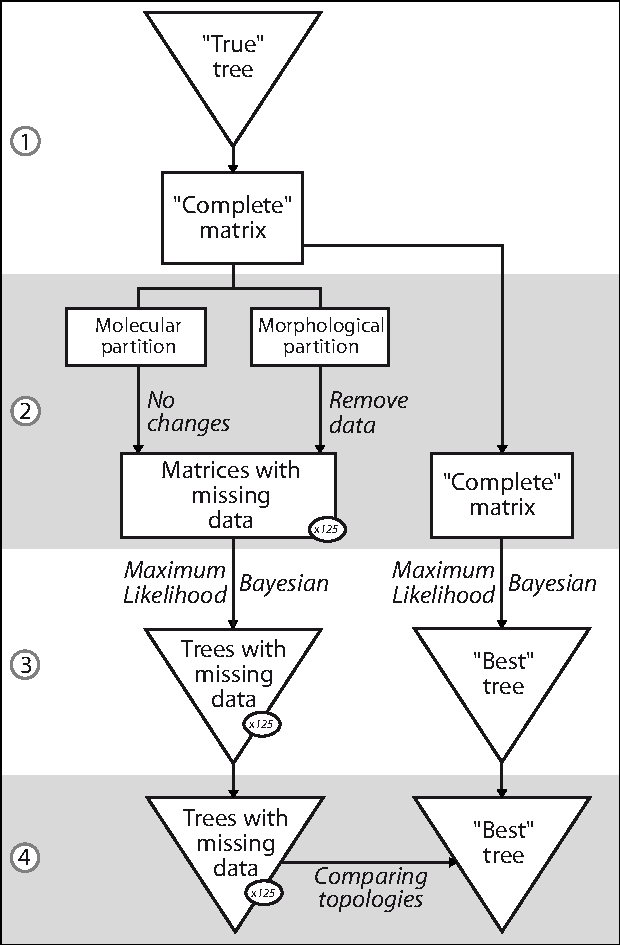
\includegraphics[width=1\textwidth]{TEM/Figures/Fig1.pdf}
\caption[Protocol outline]{\textbf{Protocol outline.}
(1) We randomly generated a birth-death tree (the ``true'' tree) and used it to simulate a matrix with no missing data (the ``complete'' matrix).
(2) We removed data from the morphological part of the ``complete'' matrix resulting in 125 ``missing-data'' matrices.
(3) We built phylogenetic trees from each matrix using both Maximum Likelihood and Bayesian methods.
(4) We compared the ``missing-data'' trees to the ``best'' tree.
We repeated these four steps 50 times.}
\label{Fig_Outline}
\end{figure}

%---------------------------------------------
%       1-Generating the matrix
%---------------------------------------------

\subsection{Generating the matrix}
\label{Generating_the_matrix}
First we randomly generated a ``true'' tree of 50 taxa in R v. 3.0.2 \citep{R} using the package diversitree v. 0.9-6 \citep{fitzjohndiversitree2012}.
We generated the tree using a birth death process by sampling speciation ($\lambda$) and extinction ($\mu$) rates from a uniform distribution (bounded between 0 and 1) but maintaining $\lambda$ $>$ $\mu$ \citep{paradistime-dependent2011}.
Empirical Total Evidence matrices vary in whether they have more fossil than living taxa or vice versa.
For example, fossil taxa make up 88\% \citep{beckancient2014}, 58\% \citep{schragocombining2013}, 48\% \citep{pyrondivergence2011}, 31\% \citep{ronquista2012} and 31\% \citep{slaterphylogenetic2013} of taxa in various studies.
To avoid biasing our simulations towards either living or fossil taxa and to make each simulation comparable, we implemented a rejection sampling algorithm to select only trees with 25 living and 25 fossil taxa.
The fossil taxa were considered as unique tips at the end of extinct lineages.
We then added an outgroup to the tree, using the mean branch length of the tree to separate the outgroup from the rest of the taxa, and with the branch length leading to the outgroup set as the sum of the mean branch length and the longest root-to-tip length of the tree.

Next, we generated a molecular and a morphological matrix from the ``true'' tree.
The molecular matrix was simulated from the ``true'' tree using the R package phyclust v. 0.1-14 \citep{chen2011}.
The matrix contained 1000 character sites for 51 taxa and was generated using the seqgen algorithm \citep{ranbaut1997seqgen} and using the HKY model \citep{HKY85} with random base frequencies (sampled from a uniform probability distribution bounded between 0 and 1 with the total frequency for the four bases equal to 1) and transition/transversion rate of two \citep{douadycomparison2003}.
The substitution rates were selected from a gamma distribution with an ($\alpha$) shape of 0.5 \citep{yangamong-site1996}.
In practice, a value of $\alpha$ $<$ 1 decreases the number of sites with high substitution rates, thus reducing homoplasic sites and increasing the phylogenetic signal \citep{Hassanin1998611,EstoupHomoplasy}.
Also, we chose this $\alpha$ value to be consistent with our protocol for simulating morphological characters (see below).
This model and these parameter settings strike a balance between realism for empirical datasets \citep[e.g.][]{douadycomparison2003,kellymolecular2014} and parameter richness with more complex models (e.g., GTR, multiple partitions with independent models), making them more suitable for our computational limitations (even with the parameters defined, the total computational time for the whole analysis was around 150 CPU years).
All the molecular information for fossil taxa was replaced by missing data ("?").

We simulated the morphological matrix using the rTraitDisc function from the R package ape v. 3.0-11 \citep{paradisape:2004} to generate a matrix of 100 character sites for 51 taxa.
We assigned the number of character states (either two or three) for each morphological character by sampling with a probability of 0.85 for two states characters and 0.15 for three state characters.
We extracted these values from 100 random empirical matrices with more than 100 characters each downloaded from TreeBASE (\url{http://treebase.org/}).
We selected matrices published between 1985 and 2013 and covering 19 taxonomic classes (Chordata, Arthropoda, Annelida, Angiosperm, Gymnosperm and Pteridophyta).
These matrices contained a cumulative number of 22563 characters that had between two and 10 character states.
We then extracted the proportion of characters with each number of states (two to 10) to give us an empirical estimate of the average number of character states for each character, as shown in Fig. \ref{Fig_AppendixCharacters}.
Most morphological characters have two or three states, therefore we only simulate characters with two or three states, and sampled these in proportion to their occurrence in our empirical data (probability of 0.85 for two states characters and 0.15 for three state characters).

\begin{figure}[!htbp]
\centering
    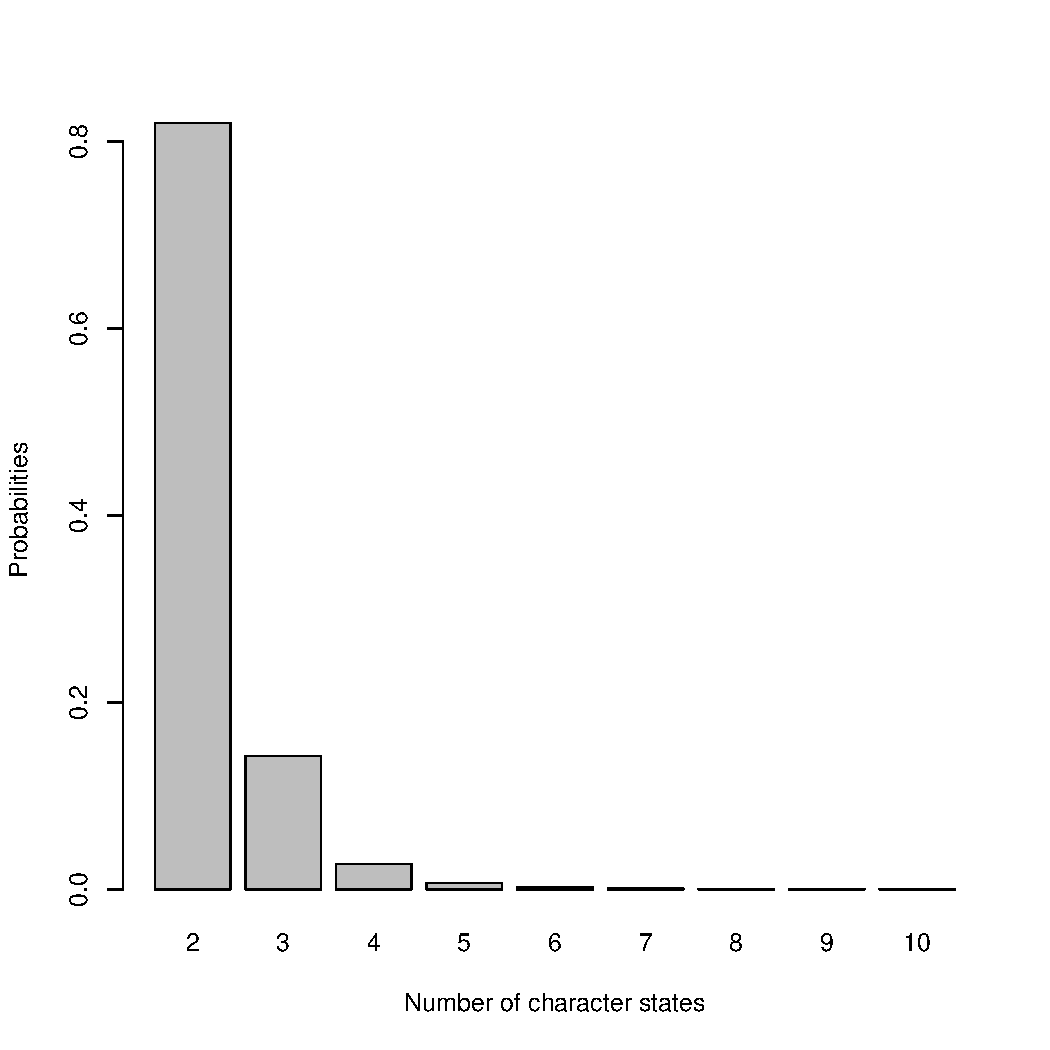
\includegraphics[keepaspectratio=true]{TEM/Figures/TEM_Fig-AppendixCharacters.pdf}
\caption{The proportion of morphological characters with between two and 10 character states extracted from 100 randomly selected empirical matrices downloaded from TreeBASE.}
\label{Fig_AppendixCharacters}
\end{figure}

We then ran an independent discrete character simulation for each character using the ``true'' tree with the character's randomly selected number of states (two or three) and assuming an equal rate of change (i.e. evolutionary rate) from one character state to another \citep{Pagel22011994}.
This method allows us to have only two parameters for each character: the number of states and the evolutionary rate.
For each character, the evolutionary rate was sampled from a gamma distribution with $\alpha$ = 0.5.
We used low evolutionary rate parameters to be consistent with the molecular rate parameters, to avoid homoplasy in the morphological part of the matrix and create a clear phylogenetic signal \citep{wrightbayesian2014}.
Topological error has been shown to be minimal at a morphological rate of 0.5 when using the M\textit{kv} model \citep{lewisa2001,wrightbayesian2014}.
Note, however, that \cite{wrightbayesian2014} have shown that low morphological rates ($<$ 0.5) increase variance in topological error, but we discarded simulations with such topological error by selecting only matrices with a ``fair'' phylogenetic signal \citep[see Estimating phylogenies section below;][]{zanderminimal2004} so this should not influence our results.

Finally, we combined the morphological and molecular matrices obtained from the ``true'' tree.
Hereafter we call this the ``complete'' matrix, i.e. the matrix with no missing data except for the molecular data of the fossil taxa.

%---------------------------------------------
%       2-Removing data
%---------------------------------------------

\subsection{Removing data}
To explore the effect of missing morphological data on topological recovery, we removed various amounts of the ``complete'' matrix to obtain matrices with missing morphological data.
Hereafter, we call these matrices with missing morphological data the ``missing-data'' matrices.
Note that the amount of molecular data remained constant throughout our simulations: 1000 molecular characters for living taxa and no molecular data for fossil taxa (see above).
We removed morphological data using three data incompleteness parameters:
\begin{enumerate}
\item{The proportion of missing living taxa ($M_L$).}
This first missing-data parameter corresponds to the proportion of living taxa with no morphological data. It represents the number of living taxa that are present in the matrix but have only molecular data available. This reflects the fact that, because of the increasing ease of collecting molecular data, morphological data for living species are rarely collected \citep{GuillermeCooperMissing}.
Therefore, many living species will have only molecular data available.
In practice, we removed all the morphological data from randomly chosen living taxa with five different proportions: 0\%, 10\%, 25\%, 50\% or 75\% of living taxa with no morphological data.
\item{The proportion of missing data in the fossil record ($M_F$).}
This missing data parameter represents the completeness of the fossil record.
Due to preservation biases, missing data for fossil taxa are common \citep{sansomfossilization2013}.
In practice, we randomly removed a proportion of data from across the fossil taxa with five different proportions: 0\%, 10\%, 25\%, 50\% or 75\% of overall missing data for the fossil taxa.
Note that 50\% missing data for fossil taxa does not mean that each fossil is missing 50\% of its morphological data.
Instead this 50\% refers to missing fossil data across the whole matrix.
Some fossils may retain 100\% of their data and others may lose most of their data at this parameter value (down to a minimum threshold of 5\% available data; see below).
\item{The number of morphological characters for both living and fossil taxa ($N_C$).}
This parameter is not a missing data parameter \textit{per se} but rather an indication of the size of the matrix.
Any morphological matrix of any size has indeterminate missing data, given that the total number of characters is undefined, but presumably large.
Therefore, this parameter corresponds to the overall number of characters available for both living and fossil taxa.
In practice, we randomly removed entire characters from the morphological matrix reducing it to: 100, 90, 75, 50 or 25 characters.
Note that these levels are equivalent to the two other parameters (i.e. 0\%, 10\%, 25\%, 50\% or 75\% of ``missing'' morphological characters).
\end{enumerate}

Each parameter represents a different way of removing data from the morphological part of the matrix: $M_L$ removes entire rows from the living data; $M_F$ removes cells from the fossil data; and $N_C$ removes columns across both living and fossil data.
Note that $M_L$ and $M_F$ differ not only because of the region of the matrix affected: for $M_L$ all the morphological data of a percentage of living taxa are removed, whereas for $M_F$ a percentage of the data are removed at random from across the whole of the morphological matrix for fossil taxa.

We created matrices using all parameter combinations resulting in 125 ($5^3$) ``missing-data'' matrices.
Note that one of these combinations ($M_L$=0\%; $M_F$=0\% and $N_C$=100) has no missing data so is equivalent to the ``complete'' matrix, thus we have one effectively complete matrix in our 125 ``missing-data'' matrices.
In practice, we first removed the data following the two missing data parameters $M_L$ and $M_F$ and then removed data following the $N_C$ parameters.
To avoid avoid matrices containing taxa without any data (morphological or molecular), we repeated the random deletion until the matrices contained at least 5\% of data for any taxon.
Note that the living taxa always had at least 90\% of data (the 1000 molecular characters).

%---------------------------------------------
%       3-Building phylogenies
%---------------------------------------------

\subsection{Estimating phylogenies}
From the resulting matrices we generated two types of trees: the ``best'' tree inferred from the ``complete'' matrix and the ``missing-data'' trees inferred from the 125 matrices with various amounts of missing data.
The ``true'' tree was used to generate the ``complete'' matrix and reflects the ``true'' evolutionary history in our simulations.
The ``best'' tree, on the other hand, is the best tree we can build using state-of-the-art phylogenetic methods.
In real world situations, the ``true'' tree is never available to us because we cannot know the true evolutionary history of a clade \citep[except in very rare circumstances, e.g.][]{rozen2005}.
We compare ``best'' trees to ``missing data'' trees but could also compare ``true'' trees to the ``missing data'' trees.
In practice, the difference between the ``best'' trees and the ``missing data'' trees represents the effect of our missing data parameters and of the phylogenetic methods used to infer the ``missing data'' trees.
The difference between the ``true'' and the ``missing data'' trees, however, represents the effect of our parameters used to generate the ``true'' tree and the algorithms used to generate the ``complete'' matrix as well as the effect of our missing data parameters and the phylogenetic methods used.
Because the main aim of this study is to look at the effect our missing data parameters on topological recovery, we chose to represent only the comparisons between the ``best'' trees and ``missing data'' trees.
The results of the comparisons of the ``true'' tree and the ``missing data'' trees are available in Supplementary data A.1. %link?
Note that this makes little difference to our overall results.

\subsubsection*{Maximum Likelihood}
The ``best'' tree and the ``missing-data'' trees were inferred using RAxML v. 8.0.20 \citep{Stamatakis21012014}. For the molecular data, we used the GTR + $\Gamma_4$ model (\citealp{tavare1986}; default GTRGAMMA in RAxML v. 8.0.20; \citealp{Stamatakis21012014}).
For the morphological data, we used the M\textit{kv} model \citep{lewisa2001} assuming an equal state frequency and a unique overall substitution rate ($\mu$) following a gamma distribution of the rate variation with four distinct categories (M\textit{kv} + $\Gamma_4$; -K MK option in RAxML v. 8.0.20; \citealp{Stamatakis21012014}).
We used RAxML because it automatically corrects for acquisition bias \citep{lewisa2001}. It is also heavily used in the literature for Maximum Likelihood tree inference \citep[e.g.][]{rouresite-specific2011,Bogdanowicz2012,springermacroevolutionary2012,O'Leary08022013,kellymolecular2014} and is one of the fastest methods available \citep{Stamatakis01102008}. 

To measure the support for each branch in our simulated phylogenies we first ran a fast bootstrap analysis (Lazy Sub-tree Rearrangement) with 500 replicates on the ``complete'' matrix.
We removed all the simulations with a median bootstrap support lower than 50 as a proxy for weak phylogenetic signal \citep{zanderminimal2004}.
We repeated this selection until we obtained 50 sets of simulations (i.e. 50 ``complete'' and 50 x 125 ``missing-data'' matrices) with a relatively strong phylogenetic signal (median bootstrap $>$ 50).
This step was implemented to make sure that the differences we observed in topologies (see below) were due to the amount of missing data for each parameter ($M_L$, $M_F$ and $N_C$) and not simply to low branch support that is likely to lead to different topologies.
On these selected simulations, we used the fast bootstrap algorithm and performed 1000 bootstraps for each tree inference to assess topological support \citep{pattengale2010many}.
Using these parameters took \texttildelow 8 CPU years to build 50 sets of 125 bootstrapped Maximum Likelihood trees (2.30GHz clock speed nodes). We performed this procedure to increase the resolution of our resulting trees. 

\subsubsection*{Bayesian Inference}
The ``best'' tree and the ``missing-data'' trees were inferred using MrBayes v. 3.2.1 \citep{Ronquist2012mrbayes}.
We partitioned the data to treat the molecular part as a non-codon DNA partition and the morphological part as a multi-state morphological partition.
The molecular evolutionary history was inferred using the HKY model with a transition/transversion ratio of two \citep{douadycomparison2003} and a gamma distribution for the rate variation with four distinct categories (HKY + $\Gamma_4$).
For the morphological data, we used the M\textit{kv} model \citep{lewisa2001}, with equal state frequency and a unique overall substitution rate ($\mu$) with four distinct rates categories (M\textit{kv} + $\Gamma_4$).
Note that MrBayes automatically corrects for acquisition bias in the morphological data partition \citep{Nylander01022004,Ronquist2012mrbayes}.
We chose these models to be consistent with the parameters used to generate the ``complete'' matrix.

Each Bayesian tree was estimated using two runs of four chains each for a maximum of 5$\times$$10^7$ generations.
For each estimation, we used the ``true'' tree's topology as a starting tree (with a starting value for each branch length of one).
We used a fixed starting tree rather than a random starting tree \citep[default MrBayes;][]{Ronquist2012mrbayes} to speed up our Bayesian inferences.
To assess if this had an effect on the topology of the ``best'' tree, we ran a sub-sample of trees using a different random starting tree for the two MCMC chains \citep[default MrBayes option;][]{Ronquist2012mrbayes}.
We tested this effect on five trees with the five levels of missing data (i.e. first tree: $M_L$=0\%, $M_F$=0\% and $N_C$=100 (i.e. 0\% ``missing''); second tree: $M_L$=10\%, $M_F$=10\% and $N_C$=90, etc.) on the first 20 simulation chains.
We then compared the trees inferred using a random starting tree to the ``best'' tree using the normalised Robinson-Foulds and Triplets metrics in an identical way as described below (Fig. ~\ref{Fig_startingTree}).

\begin{figure}[!htbp]
\centering
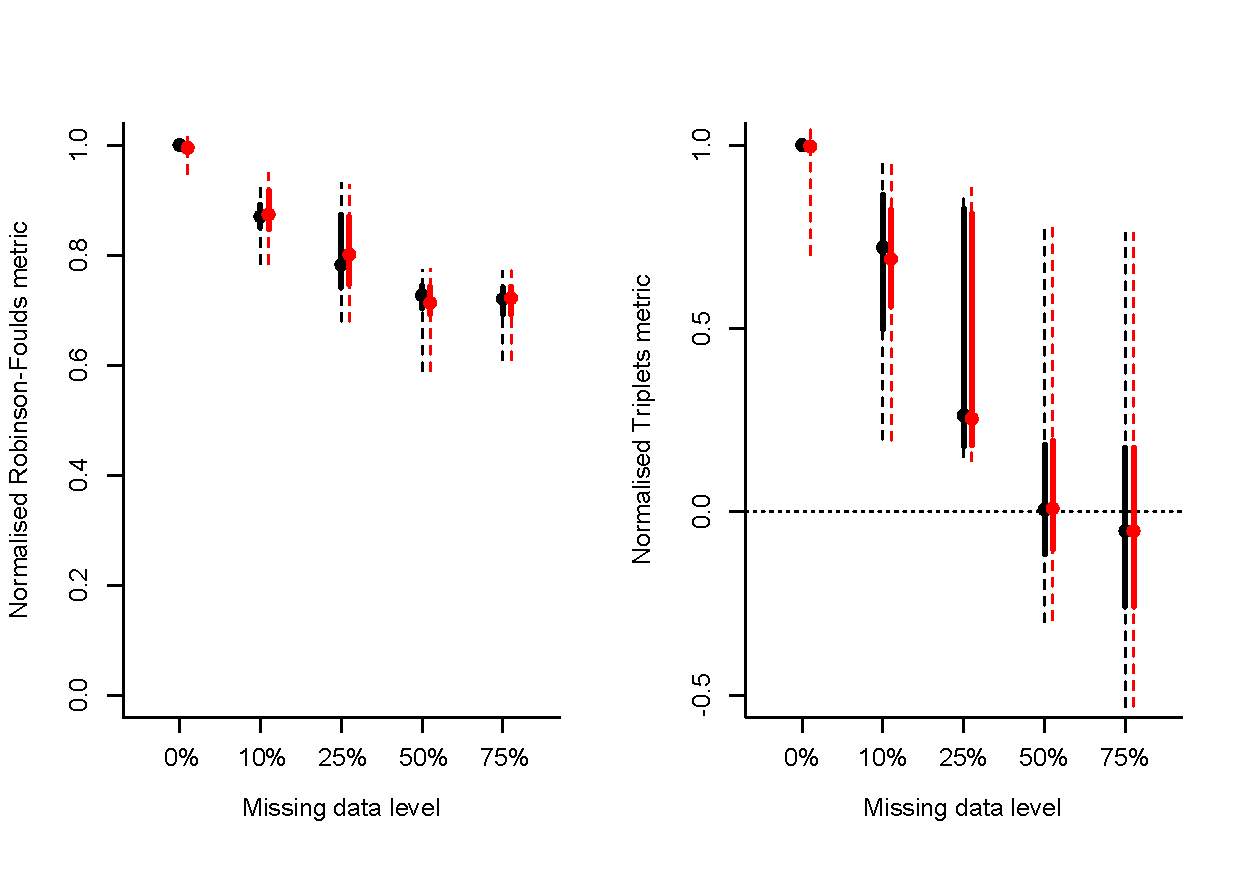
\includegraphics[keepaspectratio=true, width=\textwidth]{TEM/Figures/Starting_tree.pdf}
\caption{Effect of using the ``true'' tree (black) or a random tree (red) as the starting tree for the Bayesian inference. The x axis, represents the amount of missing data (see below).}
\label{Fig_startingTree}
\end{figure}

We used a two-way ANOVA to test any significant effect of the starting tree (``true'' or random) on the normalised Robinson-Foulds and Triplets metrics.
We found no significant effect of using the ``true'' instead of a random tree as a starting tree on our ability to recover the ``best'' tree (Table ~\ref{Tab_lm_res}).

\begin{table}[ht]
\caption[Effect of using the ``true'' tree as a starting tree]{Test of the effect of using either a random tree or the ``true'' tree as a starting tree on two Normalised Robinson-Foulds (RF) and Triplets (Tr) metrics using a two-way ANOVA.}
\label{Tab_lm_res}
\centering
\begin{tabular}{rlcccccc}
  \hline
 metric & terms & Df & Sum Sq & Mean Sq & F value & Pr($>$F) \\ 
  \hline
RF & starting    & 1 & 0.00 & 0.00 & 0.01 & 0.9125 \\ 
   & Residuals   & 198 & 2.97 & 0.01 &  &  \\ 
Tr & starting    & 1 & 0.01 & 0.01 & 0.07 & 0.7887 \\ 
   & Residuals   & 198 & 34.57 & 0.17 &  &  \\ 
   \hline
\end{tabular}
\end{table}

Note that these results are not surprising since a starting tree is not a Bayesian prior on topology \textit{per se}.

Additionally, we used two priors on the molecular part of the matrix: an exponential prior on the shape of the gamma distribution of $\alpha$ = 0.5, and a transition/transversion ratio prior of two sampled from a strong beta distribution ($\beta$(80,40)); and one prior on the morphological part of the matrix (exponential prior on the shape of the gamma distribution of $\alpha$ = 0.5).
We used these priors to speed up the Bayesian estimation process.
These priors biased the way the Bayesian process calculated branch lengths by giving non-random starting points and boundaries for parameter estimation however, here we are focusing on the effect of missing data on tree topology and not branch lengths.
Even using these priors, it took $~$ 140 CPU years to build 50 sets of 125 Bayesian trees (2.30GHz clock speed nodes).
The detailed MrBayes parameters are available in Supplementary data A.2. %link
We also included an analysis showing the effect of missing data on the estimation of the shape parameter ($\alpha$) of the morphological substitution rate distribution.
This extra analysis, however, is beyond the scope of this paper so the results are not discussed further here.

We used the average standard deviation of split frequencies (ASDS) as a proxy to estimate the convergence of the chains and used a stop rule when the ASDS went below 0.01 \citep{Ronquist2012mrbayes}.
We also checked the effective sample size (ESS) on a random sub-sample of runs in each simulation to ensure that ESS $>>$ 200 \citep{drummond2006ess}.
Finally we built a strict majority rule Bayesian consensus tree from the combined chains, excluding the 25\% first iterations as burn-in \citep{Ronquist2012mrbayes}.

%---------------------------------------------
%       4. Comparing Topologies
%---------------------------------------------

\subsection{Comparing topologies}
We compared the topology of the ``missing-data'' trees to the ``best'' tree to measure the effect of the three parameters $M_{L}$, $M_{F}$ and $N_{C}$ on tree topology.
We used the Robinson-Foulds distance \citep{RF1981} to assess the number of conserved clade positions and the Triplets distance \citep{dobson1975triplets} to assess the number of wildcard taxa \citep[i.e. taxa that frequently change position in different trees][]{kearneyfragmentary2002}. We used these two metrics because they illustrate two different aspects of tree topology (see Discussion) but also because their performance in measuring differences in topology is well described \citep{Kuhner04112014} and well implemented \citep{Bogdanowicz2012}.
We normalised both metrics using methods described in \citet{Bogdanowicz2012} to generalize our results for any \textit{n} number of taxa.
These metrics are described in detail below.

\subsubsection*{Robinson-Foulds distance}
The Robinson-Foulds distance \citep{RF1981}, or ``path difference", measures the difference between the number of clades and twice the number of shared clades across two trees.
The metric reflects the distance between the distributions of tips among clades in the two trees \citep{RF1981}:
\begin{equation}
RF_{x,y} = N_{x} + N_{y} - 2C_{x,y}
\end{equation}
where $C_{x,y}$ is the number of clades in common in the two trees.
$C$ is equal to one if the two trees have the same $n$ taxa; and $C = n-2$ when none of the $n$ taxa are shared between the trees.
This metric is bounded between zero, when the two trees are identical, and $2(n-2)$ (for two trees with $n$ taxa) when there is no shared clade in the two trees.
This metric is sensitive to minor changes in clade conservation: if the trees are composed of two clades of three taxa \textit{(((a,b),c),((d,e),f))}, the swapping of any two taxa will lead to a maximal score of the Robinson-Foulds distance indicating poor tree similarity.

We normalised this metric following Bogdanowicz's Normalised Tree Similarity (NTS) method \citep{Bogdanowicz2012}.
For any tree with \textit{n} taxa compared using a tree difference metric $m$, Normalized Tree Similarity, $NTS_m$, represents the similarity score for the two trees given the expected difference between 1000 random Yule trees \citep{Bogdanowicz2012} with $n$ taxa. If $\bar{d}_{m,n}$\textit{(rand)} is the average difference between two random Yule trees with $n$ taxa and $d_{m,n}$\textit{(x,y)} the difference between the two trees \textit{x} and \textit{y} each containing $n$ taxa, then:
\begin{equation}
NTS_{m,n}(x,y)=\frac{\bar{d}_{m,n}(rand) - d_{m,n}(x,y)} {\bar{d}_{m,n}(rand)}
\end{equation}
\textit{NTS} ranges from one to -$\infty$.
For any $m,n$, when $NTS$ = 1, the trees are identical, when \textit{NTS} = 0 the trees are no more different than expected by chance, and when $NTS$ $<$ 0, the trees are more different than expected when comparing two random trees. 

This method is a generalisation of the topological accuracy method \citep{Price2010} allowing to compare topological differences between any tree with any tree comparison metric.
In practice when the Normalised Robinson-Foulds metric between two trees is equal to one, the trees are identical; if the metric is equal to zero, the trees are no more different than expected by chance; finally if the metric is less than zero, the trees are more different than expected by chance.
Note that once rescaled, the Normalised Robinson-Foulds metric is a measure of similarity, rather than of distance like the original Robinson-Foulds metric. 

\subsubsection*{Triplets distance}
The Triplets distance \citep{dobson1975triplets} measures the number of sub-trees made up of three taxa that differ between two trees \citep{critchlowthe1996}:
\begin{equation}
S_n = \sum_{ijk} I_{ijk}
\end{equation}
where:
\begin{equation}
\sum_{ijk} = \binom{n}{4} = \frac{n!}{4!(n-4)!}
\end{equation}
and where \textit{n} is the total number of taxa in both trees (modified from \cite{critchlowthe1996}).
If $S_n$ = 0, the trees are identical; when $S_n$ = $\binom{n}{4}$, the trees are as different as possible (i.e. every taxon has a different placement in the two trees).
This metric measures the position of each taxon and clade in relation to its closest neighbours.
It is bounded between zero when the two trees are identical and $\binom{n}{3}$ (for two trees with $n$ taxa) when there is no shared taxa/clade position in the two trees.
Therefore this metric is sensitive to the conservation of wildcard taxa.
We normalised this metric in the same way as for the Robinson-Foulds distance resulting in the Normalised Triplets metric.

\subsubsection*{Paired tree comparisons}
\label{tree_comparisons}
For the Maximum Likelihood and Bayesian consensus trees we performed pairwise comparisons between the ``best'' tree and each ``missing-data'' tree using both the Normalised Robinson-Foulds and Normalised Triplets metrics with the TreeCmp java script \citep{Bogdanowicz2012} resulting in 125 Normalised Robinson-Foulds metrics and 125 Normalised Triplets metric for each tree inference method.
Also, to take into account the uncertainty of tree inference, we extracted 1000 random bootstrapped trees from the Maximum Likelihood analysis and 1000 trees from the posterior tree distribution of the Bayesian analysis for the ``best'' trees, and then did the same for the 125 ``missing data" trees (resulting in 1000 ``best'' trees and 125$\times$1000 ``missing data" trees). 
For a given set of 1000 ``missing data" trees and the 1000 ``best'' trees, we sampled one ``missing data" tree and one ``best'' tree at random and compared them using both the Normalised Robinson-Foulds and Normalised Triplets metrics as described above.
We repeated this 1000 times for each set of ``missing data" trees resulting in 125$\times$1000 values for each metric.
We repeated all the paired tree comparisons described above for each of the 50 simulation runs.
We then calculated the mode and the 50\% and 95\% confidence intervals from the resulting distribution using the hdrcde R package v. 3.1 \citep{hdrcde}.

\subsection{Testing the effects of the missing data parameters on topological recovery}
Finally, we tested the effects of our missing data parameters ($M_{L}$, $M_{F}$, $N_{C}$ and their interactions) on our ability to recover the ``best'' tree topology in a Total Evidence framework.
We also assessed the effect of our missing data parameters jointly with the effects of different tree inference and uncertainty methods (i.e. Maximum Likelihood, Bayesian consensus, Maximum Likelihood bootstrap trees and Bayesian posterior tree distribution).

We measured similarities among the distributions of the different metrics scores (Normalised Robinson-Foulds and Normalised Triplets metric) using the Bhattacharyya Coefficient \citep{Bhattacharyya}.
The Bhattacharyya Coefficient is the probability of overlap between two distributions bounded between 0 (no overlap) and 1 \citep[full overlap;]{Bhattacharyya}.
The coefficient is calculated as the sum of the square root of the relative counts shared in \textit{n} bins among two distributions.
\begin{equation}
\text{Bhattacharyya Coefficient}=\sum_{i=1}^{n} \sqrt{{\sum{a_i}}\times{\sum{b_i}}}
\end{equation}
where
\begin{equation}
{a_i}=\frac{\text{Number of counts in bin \textit{i} for the distribution \textit{a}}}{\text{Total number of counts for the distribution \textit{a}}}
\end{equation}
and
\begin{equation}
{b_i}=\frac{\text{Number of counts in bin \textit{i} for the distribution \textit{b}}}{\text{Total number of counts for the distribution \textit{b}}}
\end{equation}
The precision of the Bhattacharyya Coefficient is directly related to the number of bins, $n$. If $n$ is low, the overlap will be overestimated and if $n$ is too high, the overlap will be underestimated. In this analysis, we determined the number of bins using Silverman's rule of thumb which states that $n$ should be 0.9 times the minimum of the standard deviation and the interquartile range of the distribution, divided by 1.34 times the sample size of the distribution to the negative one-fifth power (\texttt{bw.nrd0()} function in R \citep{silverman1986density}).
When the Bhattacharyya Coefficient between two distributions is $<$0.05, the distributions are significantly different.
When this coefficient is $>$0.95 both distributions are significantly similar.
Values in between these two threshold just show the probability of overlap between the distributions but are not conclusive to assess the similarity or differences between the distributions.

Note that this is comparable to performing a two-sided t-test, but we use the Bhattacharyya Coefficient here because we are comparing whole distributions not just their means.
When the Bhattacharyya Coefficient between two distributions is $<$0.05, the distributions are significantly different.
When this coefficient is $>$0.95, the distributions are significantly similar.
Values between these two thresholds show the probability of overlap between the distributions but do not allow us to define the significance of the similarity or differences between distributions.
To assess the effect of our missing data parameters, we calculated the Bhattacharyya Coefficient between the distributions of the different metrics scores (Normalised Robinson-Foulds and Normalised Triplets metric) for each pairwise combination of missing data parameters ($M_{L}$, $M_{F}$, $N_{C}$) and parameter states (0\%, 10\%, 25\%, 50\%, 75\% and 100, 90, 75, 50, 25 characters), i.e. $M_{L}$ = 0\%, $M_{F}$ = 0\%, $N_{C}$ = 100; $M_{L}$ = 10\%, $M_{F}$ = 0\%, $N_{C}$ = 100 etc. (see Fig. \ref{Fig_Bhattacharyya_Coefficients1} for more details).
This resulted in 7875 pairwise comparisons (a triangular matrix with $3^5$$\times$$3^5$ cells).
We performed this procedure separately for each tree inference and uncertainty method.
When two combinations of missing data parameters have a similar ability to recover the ``best'' tree topology the Bhattacharyya Coefficient will be close to one.
Conversely, if the two combinations of missing data parameters differ, the Bhattacharyya Coefficient will be close to zero.
Because of the difficulties in representing so many pairwise comparisons in a meaningful way, we summarized these results as a heat map of Bhattacharyya Coefficients (see Fig. \ref{Fig_Results-paircomp_within}).
In this type of figure, parameters that have similar effects on recovering the ``best'' topology (either positive or negative effects) will be denoted by similar colour patches in the heat map representation of these comparisons (see Fig. \ref{Fig_Results-paircomp_within}).

\begin{figure}[!ht]
\centering
    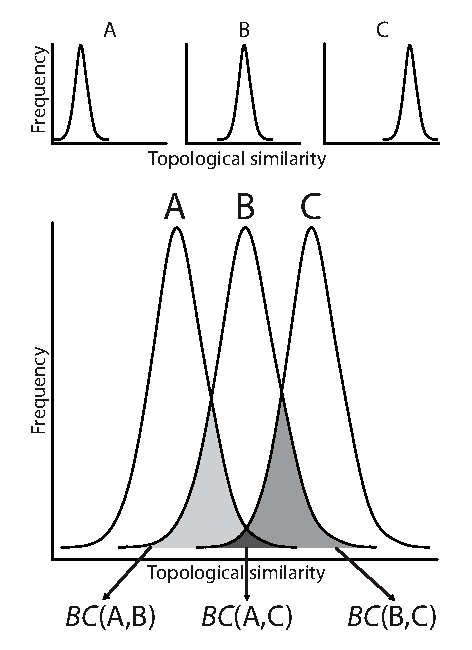
\includegraphics[width=0.5\textwidth]{TEM/Figures/Fig2.pdf}
\caption[Bhattacharyya Coefficient calculation outline 1]{\textbf{Bhattacharyya Coefficient calculation outline 1.} A, B and C are distributions of tree similarity metrics (Normalised Robinson-Foulds or Normalised Triplets metrics) for any combination of missing data parameters (e.g. $M_{L}$ = 10\%, $M_{F}$ = 50\%, $N_{C}$ = 25). The Bhattacharyya Coefficient (BC) is the overlap of the distribution of tree similarity metrics between two combinations of missing data parameters, for example, BC(A,B) is the probability of overlap between the distributions A and B.}
\label{Fig_Bhattacharyya_Coefficients1}
\end{figure}

To assess the effect of the different tree inference and uncertainty methods (i.e. Maximum Likelihood, Bayesian consensus, Maximum Likelihood bootstrap trees and Bayesian posterior tree distribution) on our ability to recover the ``best'' tree topology, we calculated the Bhattacharyya Coefficient between the distributions of the different metrics scores (Normalised Robinson-Foulds and Normalised Triplets metric) for each pairwise combination of tree inference and uncertainty methods, i.e. Maximum Likelihood \textit{versus} Bayesian consensus; Maximum Likelihood \textit{versus} Maximum Likelihood bootstrap trees etc. (see Fig. \ref{Fig_Bhattacharyya_Coefficients2} for more details).
Note that this procedure pools results from across all missing data parameter combinations so it results in just six pairwise comparisons.
When two tree inference or uncertainty methods have a similar ability to recover the ``best'' tree topology the Bhattacharyya Coefficient will be close to one.
Conversely, if the two tree inference or uncertainty methods differ, the Bhattacharyya Coefficient will be close to zero.

\begin{figure}[!ht]
\centering
    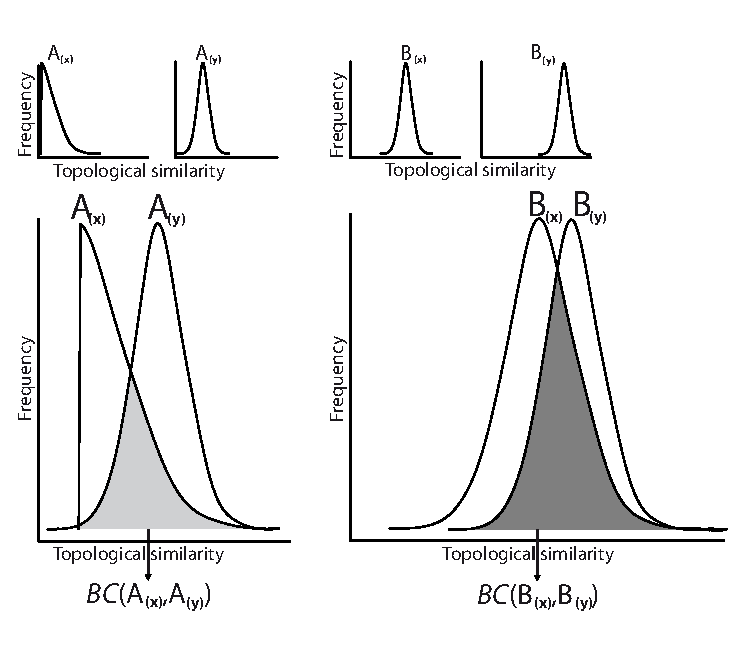
\includegraphics[width=1\textwidth]{TEM/Figures/Fig3.pdf}
\caption[Bhattacharyya Coefficient calculation outline 2]{\textbf{Bhattacharyya Coefficient calculation outline 2.} A and B are distributions of tree similarity metrics (Normalised Robinson-Foulds or Normalised Triplets metrics) for any combination of missing data parameters (e.g. $M_{L}$ = 10\%, $M_{F}$ = 50\%, $N_{C}$ = 25). \textbf{(x)} and \textbf{(y)} are two different tree inference methods (e.g. Maximum Likelihood or Bayesian). The Bhattacharyya Coefficient (BC) is the overlap of the distribution of tree similarity metrics between two methods for the same combination of missing data parameters, for example, BC($A_{x}$,$A_{y}$) is the probability of overlap of the distribution A for methods $x$ and $y$.}
\label{Fig_Bhattacharyya_Coefficients2} 
\end{figure}

%---------------------------------------------
%
%       RESULTS
%
%---------------------------------------------

\section{Results}
As the amount of missing data in the morphological part of the Total Evidence matrix increases, our ability to recover the ``best'' tree topology decreases, regardless of the missing data parameter ($M_{L}$, $M_{F}$ or $N_{C}$), the tree inference method (Maximum Likelihood or Bayesian) or the tree comparison metric used (Normalised Robinson-Foulds or Normalised Triplets metric).
Nonetheless, the different missing data parameters and tree inference methods do not affect the topology in the same way (Fig. \ref{Fig_Results-permeth_perparam} and Fig. \ref{Fig_Results-global_perparam}).

\begin{figure}[!ht]
\centering
    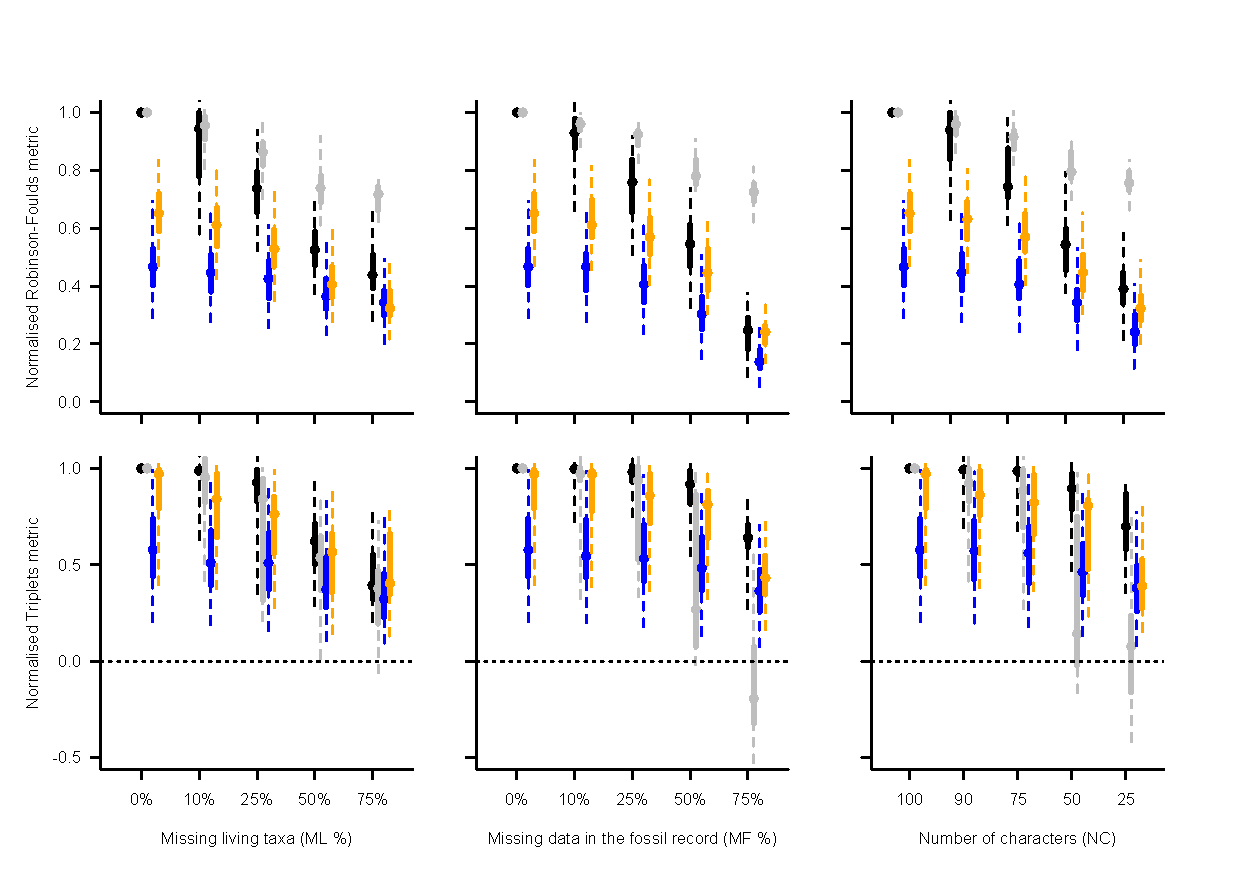
\includegraphics[width=1\textwidth]{TEM/Figures/Fig4_revised.pdf}
\caption[Effects of increasing missing data on topological recovery]{\textbf{The effects of increasing missing data on topological recovery} using Maximum Likelihood trees (black), Bayesian consensus trees (grey), Maximum Likelihood bootstrap trees (blue) and Bayesian posterior tree distributions (orange). The percentage of missing data for each parameter ($M_{L}$, $M_{F}$ and $N_{C}$) is shown on the x axis. Topological recovery was measured using two different tree comparison metrics: Normalised Robinson-Foulds metric (upper row) and Normalised Triplets metric (lower row). The graph shows the modal value (points), and the 50\% (thick solid lines) and 95\% (thin dashed lines) confidence intervals of the distributions of the tree comparison metric for each missing data parameter and tree inference method.}
\label{Fig_Results-permeth_perparam} 
\end{figure}

\begin{figure}[!ht]
\centering
    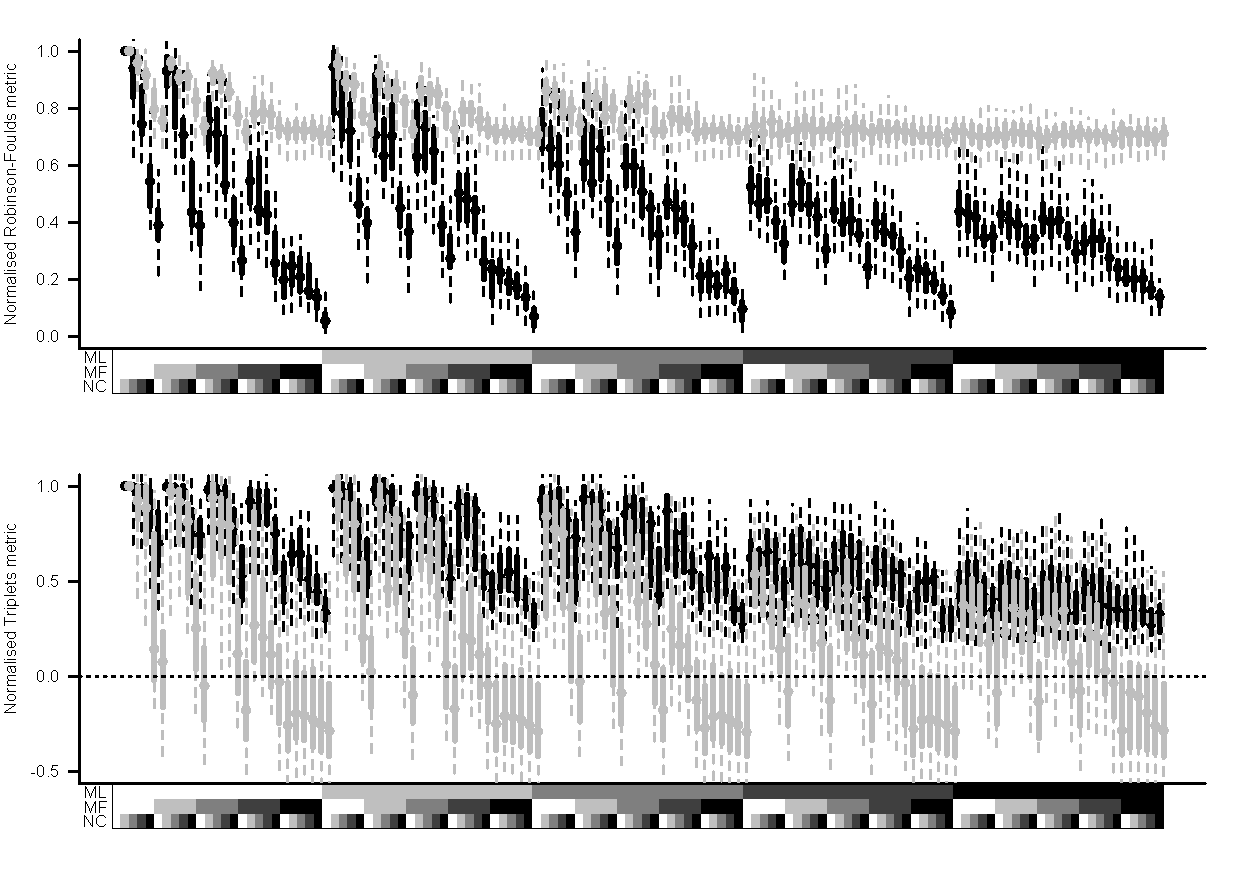
\includegraphics[width=1\textwidth]{TEM/Figures/Fig5_revised.pdf}
\caption[Effects of increasing missing data on topological recovery in Maximum Likelihood and Bayesian inference]{\textbf{The effects of increasing missing data on topological recovery using Maximum Likelihood trees (black) and Bayesian consensus trees (grey).} The x axis shows the percentage of missing data from 0\% (white) to 75\% (black) for the two parameters: $M_{L}$ (upper line), $M_{F}$ (middle line) and number of characters from 100 to 25 for the parameter $N_{C}$ (lower line). Topological recovery was measured using two different tree comparison metrics: Normalised Robinson-Foulds metric (upper row) and Normalised Triplets metric (lower row). The graph shows the modal value (points), and the 50\% (thick solid lines) and 95\% (thin dashed lines) confidence intervals of the distributions of the tree comparison metric for each missing data parameter and tree inference method.} 
\label{Fig_Results-global_perparam}
\end{figure}

\begin{figure}[!ht]
\centering
    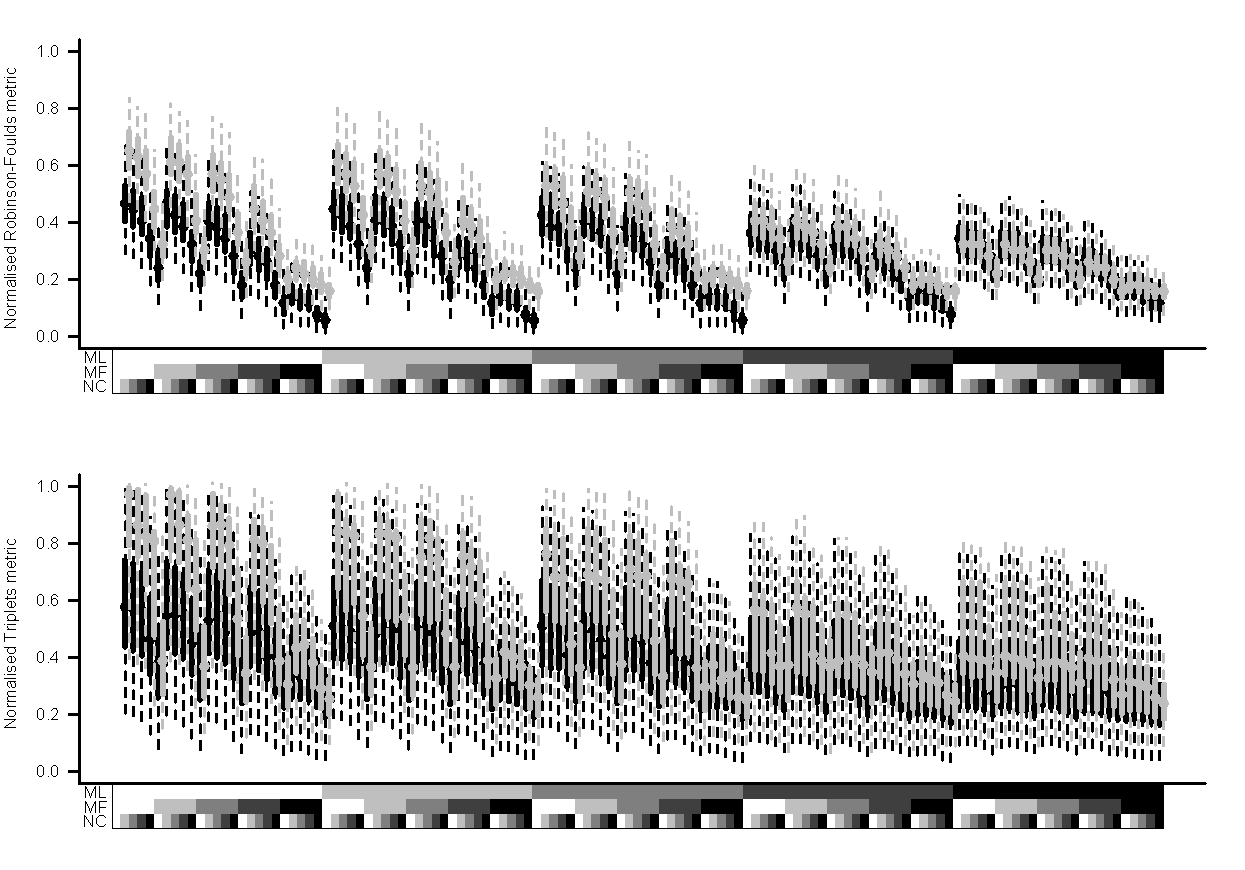
\includegraphics[width=1\textwidth]{TEM/Figures/Boot+Bayt-AllParam-RF+Tr-BW.pdf}
    \caption[Effects of increasing missing data on topological recovery on bootstrap and posterior tree distribution]{\textbf{The effects of increasing missing data on topological recovery using Maximum Likelihood Bootstrap trees (black) and Bayesian posterior tree distribution (grey)}. The x axis shows the percentage of missing data from 0\% (white) to 75\% (black) for the two parameters: $M_{L}$ (upper line), $M_{F}$ (middle line) and number of characters from 100 to 25 for the parameter $N_{C}$ (lower line). Topological recovery was measured using two different tree comparison metrics: Normalised Robinson-Foulds metric (upper row) and Normalised Triplets metric (lower row). The graph shows the modal value (points), and the 50\% (thick solid lines) and 95\% (thin dashed lines) confidence intervals of the distributions of the tree comparison metric for each missing data parameter and tree inference method.} 
\label{Fig_Supp_BootBayt_allparam} 
\end{figure}

\subsection{Individual effects of missing data parameters}
As the amount of missing data increases across all three parameters, our ability to recover the ``best'' tree topology decreases (Fig. \ref{Fig_Results-permeth_perparam}).
The Normalised Robinson-Foulds metric is always lower for the Maximum Likelihood trees than for the Bayesian consensus trees (median Bhattacharrya Coefficient = 0.69, 0.48 and 0.66 for $M_{L}$, $M_{F}$ and $N_{C}$ respectively; Fig. \ref{Fig_Results-permeth_perparam}; Tables \ref{Tab_Supp_summary_BC_ML}, \ref{Tab_Supp_summary_BC_MF} and \ref{Tab_Supp_summary_BC_MC}). 
The Normalised Triplets metric, however, is similar when comparing the Maximum Likelihood trees and the Bayesian consensus trees for all the parameters ($M_{L}$, $M_{F}$ and $N_{C}$) (median Bhattacharrya Coefficient = 0.84, 0.75 and 0.80 for $M_{L}$, $M_{F}$ and $N_{C}$ respectively; Fig. \ref{Fig_Results-permeth_perparam}; Tables \ref{Tab_Supp_summary_BC_ML}, \ref{Tab_Supp_summary_BC_MF} and \ref{Tab_Supp_summary_BC_MC}).

%Summary of the BC between pairs of methods for the ML parameter
\begin{landscape}
\begin{table}[!htb]
\caption[Bhattacharyya Coefficients of the pairwise method comparisons ($M_{L}$).]{Bhattacharyya Coefficients of the pairwise method comparisons, each of which corresponds to the normalised metric between the "best" tree and the "missing-data" using either the Normalised Robinson-Foulds metric (RF) or the Normalised Triplets metric (Tr) for the $M_{L}$ missing data parameter only.}
\label{Tab_Supp_summary_BC_ML}
\centering
\begin{tabular}{lccccccc}
  \hline
 Comparison &  Metric & Min. & 1st Qu. & Median & Mean & 3rd Qu. & Max. \\ 
  \hline
    Maximum Likelihood \textit{vs.} Bayesian consensus                 & $RF$ & 0.30 & 0.31 & 0.69 & 0.61 & 0.77 & \textbf{1.00} \\ 
                                                                       & $Tr$ & 0.79 & 0.81 & 0.84 & 0.86 & 0.85 & \textbf{1.00} \\ 
    Maximum Likelihood \textit{vs.} Maximum Likelihood bootstraps      & $RF$ & \textbf{0.03} & 0.22 & 0.29 & 0.36 & 0.54 & 0.69 \\ 
                                                                       & $Tr$ & 0.08 & 0.42 & 0.53 & 0.51 & 0.74 & 0.78 \\ 
    Maximum Likelihood \textit{vs.} Bayesian posterior trees           & $RF$ & \textbf{0.02} & 0.49 & 0.61 & 0.51 & 0.67 & 0.74 \\ 
                                                                       & $Tr$ & 0.21 & 0.61 & 0.70 & 0.63 & 0.81 & 0.81 \\ 
    Bayesian consensus \textit{vs.} Maximum Likelihood bootstraps      & $RF$ & \textbf{0.01} & \textbf{0.02} & \textbf{0.02} & \textbf{0.02} & \textbf{0.03} & \textbf{0.04} \\ 
                                                                       & $Tr$ & 0.08 & 0.69 & 0.78 & 0.64 & 0.79 & 0.84 \\ 
    Bayesian consensus \textit{vs.} Bayesian posterior trees           & $RF$ & \textbf{0.01} & \textbf{0.02} & \textbf{0.02} & \textbf{0.04} & 0.08 & 0.09 \\ 
                                                                       & $Tr$ & 0.21 & 0.74 & 0.75 & 0.68 & 0.84 & 0.87 \\ 
    Bayesian posterior tree \textit{vs.} Maximum Likelihood bootstraps & $RF$ & 0.69 & 0.75 & 0.85 & 0.85 & \textbf{0.95} & \textbf{1.00} \\ 
                                                                       & $Tr$ & 0.91 & 0.92 & \textbf{0.96} & \textbf{0.95} & \textbf{0.97} & \textbf{0.98} \\ 
   \hline
\end{tabular}
\end{table}
\end{landscape}

%Summary of the BC between pairs of methods for the MF parameter
\begin{landscape}
\begin{table}[!htb]
\caption[Bhattacharyya Coefficients of the pairwise method comparisons ($M_{F}$).]{Bhattacharyya Coefficients of the pairwise method comparisons, each of which corresponds to the normalised metric between the "best" tree and the "missing-data" using either the Normalised Robinson-Foulds metric (RF) or the Normalised Triplets metric (Tr) for the $M_{F}$ missing data parameter only.}
\label{Tab_Supp_summary_BC_MF}
\centering
\begin{tabular}{lccccccc}
  \hline
 Comparison &  Metric & Min. & 1st Qu. & Median & Mean & 3rd Qu. & Max. \\  
  \hline
    Maximum Likelihood \textit{vs.} Bayesian consensus                 & $RF$ & \textbf{0.00} & 0.25 & 0.48 & 0.50 & 0.76 & \textbf{1.00} \\ 
                                                                       & $Tr$ & 0.38 & 0.69 & 0.75 & 0.72 & 0.80 & \textbf{1.00} \\ 
    Maximum Likelihood \textit{vs.} Maximum Likelihood bootstraps      & $RF$ & \textbf{0.03} & 0.18 & 0.32 & 0.36 & 0.47 & 0.77 \\ 
                                                                       & $Tr$ & 0.08 & 0.34 & 0.40 & 0.38 & 0.53 & 0.55 \\ 
    Maximum Likelihood \textit{vs.} Bayesian posterior trees           & $RF$ & \textbf{0.02} & 0.47 & 0.71 & 0.60 & 0.86 & 0.94 \\ 
                                                                       & $Tr$ & 0.21 & 0.54 & 0.62 & 0.56 & 0.64 & 0.80 \\ 
    Bayesian consensus \textit{vs.} Maximum Likelihood bootstraps      & $RF$ & \textbf{0.00} & \textbf{0.00} & \textbf{0.01} & \textbf{0.01} & \textbf{0.01} & \textbf{0.03} \\ 
                                                                       & $Tr$ & 0.08 & 0.38 & 0.54 & 0.49 & 0.70 & 0.75 \\ 
    Bayesian consensus \textit{vs.} Bayesian posterior trees           & $RF$ & \textbf{0.00} & \textbf{0.02} & \textbf{0.02} & \textbf{0.02} & \textbf{0.04} & \textbf{0.04} \\ 
                                                                       & $Tr$ & 0.21 & 0.29 & 0.66 & 0.54 & 0.72 & 0.82 \\ 
    Bayesian posterior tree \textit{vs.} Maximum Likelihood bootstraps & $RF$ & 0.69 & 0.69 & 0.72 & 0.71 & 0.72 & 0.72 \\ 
                                                                       & $Tr$ & 0.91 & 0.91 & 0.91 & 0.93 & 0.92 & \textbf{0.98} \\ 
   \hline
\end{tabular}
\end{table}
\end{landscape}

%Summary of the BC between pairs of methods for the MC parameter
\begin{landscape}
\begin{table}[!htb]
\caption[Bhattacharyya Coefficients of the pairwise method comparisons ($N_{C}$).]{Bhattacharyya Coefficients of the pairwise method comparisons, each of which corresponds to the normalised metric between the "best" tree and the "missing-data" using either the Normalised Robinson-Foulds metric (RF) or the Normalised Triplets metric (Tr) for the $N_{C}$ missing data parameter only.}
\label{Tab_Supp_summary_BC_MC}
\centering
\begin{tabular}{lccccccc}
  \hline
 Comparison &  Metric & Min. & 1st Qu. & Median & Mean & 3rd Qu. & Max. \\  
  \hline
    Maximum Likelihood \textit{vs.} Bayesian consensus                 & $RF$ & \textbf{0.03} & 0.32 & 0.66 & 0.55 & 0.75 & \textbf{1.00} \\ 
                                                                       & $Tr$ & 0.51 & 0.69 & 0.80 & 0.76 & 0.80 & \textbf{1.00} \\ 
    Maximum Likelihood \textit{vs.} Maximum Likelihood bootstraps      & $RF$ & \textbf{0.03} & 0.17 & 0.21 & 0.31 & 0.46 & 0.68 \\ 
                                                                       & $Tr$ & 0.08 & 0.31 & 0.39 & 0.39 & 0.56 & 0.61 \\ 
    Maximum Likelihood \textit{vs.} Bayesian posterior trees           & $RF$ & \textbf{0.02} & 0.44 & 0.47 & 0.52 & 0.78 & 0.90 \\ 
                                                                       & $Tr$ & 0.21 & 0.52 & 0.59 & 0.55 & 0.66 & 0.77 \\ 
    Bayesian consensus \textit{vs.} Maximum Likelihood bootstraps      & $RF$ & \textbf{0.00} & \textbf{0.01} & \textbf{0.01} & \textbf{0.02} & \textbf{0.02} & \textbf{0.03} \\ 
                                                                       & $Tr$ & 0.08 & 0.47 & 0.62 & 0.51 & 0.66 & 0.73 \\ 
    Bayesian consensus \textit{vs.} Bayesian posterior trees           & $RF$ & \textbf{0.00} & \textbf{0.02} & \textbf{0.04} & \textbf{0.04} & 0.05 & 0.06 \\ 
                                                                       & $Tr$ & 0.21 & 0.45 & 0.64 & 0.57 & 0.74 & 0.79 \\ 
    Bayesian posterior tree \textit{vs.} Maximum Likelihood bootstraps & $RF$ & 0.69 & 0.73 & 0.73 & 0.76 & 0.81 & 0.86 \\ 
                                                                       & $Tr$ & 0.91 & 0.92 & 0.93 & 0.94 & \textbf{0.96} & \textbf{0.99} \\ 
   \hline
\end{tabular}
\end{table}
\end{landscape}

\begin{landscape}
\begin{table}[!htb]
%\begin{adjustwidth}{-2.25in}{0in} % Comment out/remove adjustwidth environment if table fits in text column.
\caption[Bhattacharyya Coefficients of the pairwise method comparisons.]{Bhattacharyya Coefficients of the pairwise method comparisons.
Each line summarizes the probabilities of overlap between the distributions of the ``best'' tree versus trees from each inference method (Maximum Likelihood; Bayesian consensus; Maximum Likelihood Bootstraps and Bayesian posterior trees) pooled across all combinations of missing data parameter values, using the Normalised Robinson-Foulds (RF) and Triplets (Tr) metrics. 
Values highlighted in bold are the extreme values of high or low probability of overlap between two methods. If two methods have a high probability of overlap, they have a similar ability to recover the ``correct'' tree topology.
Values $>$ 0.95 denote significantly similar distributions and values $<$ 0.05 denote significantly different distributions.}
\centering
\begin{tabular}{lccccccc}
  \hline
 Comparison &  Metric & Min. & 1st Qu. & Median & Mean & 3rd Qu. & Max. \\ 
  \hline
    Maximum Likelihood \textit{vs.} Bayesian consensus                 & $RF$ & \textbf{0.00} & \textbf{0.00} & 0.10 & 0.20 & 0.32 & \textbf{1.00} \\ 
                                                                       & $Tr$ & 0.34 & 0.49 & 0.61 & 0.62 & 0.75 & \textbf{1.00} \\ 
    Maximum Likelihood \textit{vs.} Maximum Likelihood bootstraps      & $RF$ & \textbf{0.03} & 0.54 & 0.69 & 0.64 & 0.77 & \textbf{0.98} \\ 
                                                                       & $Tr$ & 0.08 & 0.57 & 0.65 & 0.64 & 0.73 & 0.82 \\ 
    Maximum Likelihood \textit{vs.} Bayesian posterior trees           & $RF$ & \textbf{0.02} & 0.74 & 0.80 & 0.79 & 0.89 & \textbf{0.98} \\ 
                                                                       & $Tr$ & 0.21 & 0.67 & 0.73 & 0.72 & 0.77 & 0.84 \\ 
    Bayesian consensus \textit{vs.} Maximum Likelihood bootstraps      & $RF$ & \textbf{0.00} & \textbf{0.00} & \textbf{0.00} & \textbf{0.01} & \textbf{0.01} & \textbf{0.04} \\ 
                                                                       & $Tr$ & 0.08 & 0.38 & 0.59 & 0.57 & 0.73 & 0.84 \\ 
    Bayesian consensus \textit{vs.} Bayesian posterior trees           & $RF$ & \textbf{0.00} & \textbf{0.00} & \textbf{0.01} & \textbf{0.02} & \textbf{0.04} & 0.11 \\ 
                                                                       & $Tr$ & 0.21 & 0.36 & 0.56 & 0.55 & 0.74 & 0.87 \\ 
    Bayesian posterior tree \textit{vs.} Maximum Likelihood bootstraps & $RF$ & 0.50 & 0.77 & 0.85 & 0.85 & \textbf{0.96} & \textbf{1.00} \\ 
                                                                       & $Tr$ & 0.91 & \textbf{0.96} & \textbf{0.98} & \textbf{0.97} & \textbf{0.99} & \textbf{1.00} \\ 
   \hline
\end{tabular}
\label{Tab_Results-Difference_methods}
%\end{adjustwidth}
\end{table}
\end{landscape}


\subsection{Combined effect of missing data parameters}
As expected, our ability to recover the ``best'' tree topology is worst when each parameter contains the maximum amount of missing data (i.e. $M_{L}$ = 75\%, $M_{F}$ = 75\% and $N_{C}$ = 75\%), and best when there is no missing data (i.e. $M_{L}$ = 0\%, $M_{F}$ = 0\%, $N_{C}$ = 0\%; Fig. \ref{Fig_Results-global_perparam}; Tables \ref{Tab_Supp_summary_metric_ML}, \ref{Tab_Supp_summary_metric_MF} and \ref{Tab_Supp_summary_metric_MC}).
Fig. \ref{Fig_Results-paircomp_within} shows the similarity of distributions of tree metrics in a triangular matrix with the values of each pairwise Bhattacharyya Coefficient coloured according to their values (orange when the distributions overlap completely, Bhattacharyya Coefficient = 1, and blue when they do not, Bhattacharyya Coefficient = 0). 

\begin{figure}[!ht]
\centering
    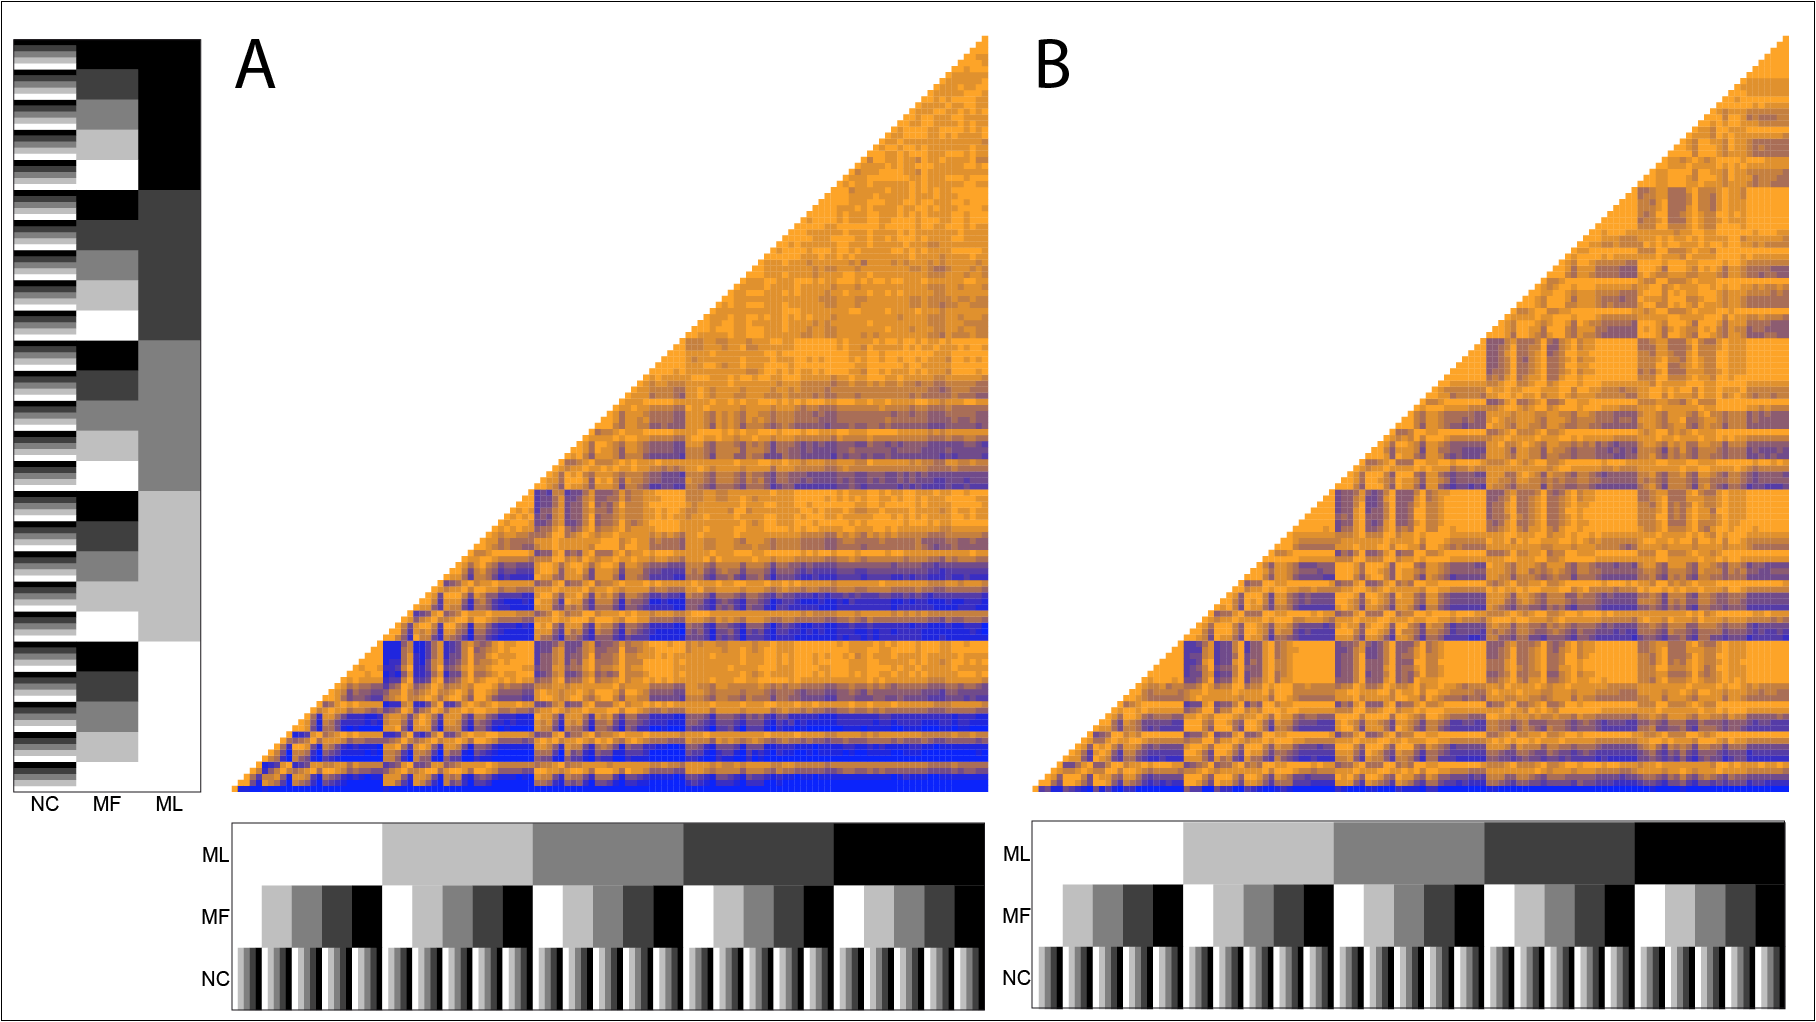
\includegraphics[width=1\textwidth]{TEM/Figures/Fig6_revised.png}
\caption[Effects of missing data on topological recovery using Bayesian consensus trees]{\textbf{The effects of missing data on topological recovery using Bayesian consensus trees.} Both axes show the percentage of missing data from 0\% (white) to 75\% (black) for the three parameters: $M_{L}$ (upper line), $M_{F}$ (middle line) and $N_{C}$ (lower line). The topological recovery is measured as (A) the Normalised Robinson-Foulds metric and (B) the Normalised Triplets metric calculated using the Bhattacharyya Coefficient. The Bhattacharyya Coefficient values are indicated using a color gradient ranging from low probability of overlap in blue, to high probability of overlap in orange. Blue regions denote a poor overlap in Normalised metric values between the different parameter combinations (i.e. the parameters have a strong effect on the metric and thus the topological recovery). Conversely, orange regions denote a high overlap in Normalised metric values between the different parameter combinations (i.e. the parameters have a weak effect on the metric and thus the topological recovery).}
\label{Fig_Results-paircomp_within}
\end{figure}

Using both Normalised Robinson-Foulds and Normalised Triplets metrics from the Bayesian consensus trees, the parameter combination with no missing data (i.e. $M_{L}$ = 0\%, $M_{F}$ = 0\%, $N_{C}$ = 100) is always the most dissimilar to all the other parameter combinations (thin deep blue line at the base of Fig. \ref{Fig_Results-paircomp_within}).
The Normalised Robinson-Foulds metric (median Bhattacharrya coefficient = 0.79; blue regions in Fig. \ref{Fig_Results-paircomp_within}A), however, displays more dissimilarities than the Normalised Triplets metric (median Bhattacharrya coefficient = 0.81; blue regions in Fig. \ref{Fig_Results-paircomp_within}B).
The orange upper triangle in Fig. \ref{Fig_Results-paircomp_within}A shows a high probability of overlap of the Normalised Robinson-Foulds metric for the trees with the $M_{L}$ parameter $\geq$ 50\% (Fig. \ref{Fig_Results-paircomp_within}A).
Once $M_{L}$ $\geq$ 50\%, there is no additional effect of $M_{F}$ and $N_{C}$, regardless of the amount of missing data in these parameters (Fig. \ref{Fig_Results-paircomp_within}A).
Likewise, once $N_{C}$ $<$ 50, there is no additional effect of $M_{L}$ and $M_{F}$ as denoted by the high probability of Normalised Robinson-Foulds metric overlap (horizontal orange stripes between the blue regions Fig. \ref{Fig_Results-paircomp_within}A).
In Fig. \ref{Fig_Results-global_perparam} for the Normalised Robinson-Foulds metric, this can be interpreted as the overlap between the distributions once $M_L$=50\%.

For all combinations of missing data parameters and tree comparison metrics, the Maximum Likelihood bootstrap trees and the Bayesian posterior tree distributions perform very similarly (median Bhattacharrya Coefficient = 0.85 and 0.98, using Normalised Robinson-Foulds metric or Normalised Triplets metric respectively; Table ~\ref{Tab_Results-Difference_methods}).
These two methods, however, perform worse than the Bayesian consensus trees using Normalised Robinson-Foulds metric (median Bhattacharrya Coefficient = 0 and 0.01, for the Maximum Likelihood bootstrap trees and the Bayesian posterior tree distribution respectively; Table ~\ref{Tab_Results-Difference_methods}; Fig. \ref{Fig_Results-permeth_perparam} and Fig. \ref{Fig_Supp_BootBayt_allparam}).

%Summary of metrics values for the ML parameter
\begin{landscape}
\begin{table}[!ht]
\caption[Summary of the tree comparisons for the $M_{L}$ parameter.]{Summary of the comparisons between the "best" tree and the "missing-data" trees for each different tree inference method using either the Normalised Robinson-Foulds metric (RF) or the Normalised Triplets metric (Tr) for the $M_{L}$ missing data parameter only.}
\label{Tab_Supp_summary_metric_ML}
\centering
\begin{tabular}{lccccccc}
  \hline
 Tree inference method & Metric & Min. & 1st Qu. & Median & Mean & 3rd Qu. & Max. \\ 
  \hline
  Maximum Likelihood                    & $RF$ & 0.44 & 0.51 & 0.63 & 0.66 & 0.78 & 0.95 \\ 
                                        & $Tr$ & 0.45 & 0.56 & 0.76 & 0.74 & 0.93 & 0.99 \\ 
  Bayesian consensus                    & $RF$ & 0.71 & 0.73 & 0.80 & 0.82 & 0.88 & 0.95 \\ 
                                        & $Tr$ & 0.37 & 0.46 & 0.67 & 0.67 & 0.87 & 0.96 \\ 
  Maximum Likelihood bootstraps         & $RF$ & 0.34 & 0.37 & 0.42 & 0.41 & 0.44 & 0.46 \\ 
                                        & $Tr$ & 0.32 & 0.40 & 0.51 & 0.46 & 0.51 & 0.57 \\ 
  Bayesian posterior tree distributions & $RF$ & 0.33 & 0.41 & 0.52 & 0.50 & 0.60 & 0.65 \\ 
                                        & $Tr$ & 0.41 & 0.56 & 0.76 & 0.71 & 0.84 & 0.98 \\ 
   \hline
\end{tabular}
\end{table}
\begin{table}[!hb]
\caption[Summary of the tree comparisons for the $M_{F}$ parameter.]{Summary of the comparisons between the "best" tree and the "missing-data" trees for each different tree inference method using either the Normalised Robinson-Foulds metric (RF) or the Normalised Triplets metric (Tr) for the $M_{F}$ missing data parameter only.}
\label{Tab_Supp_summary_metric_MF}
\centering
\begin{tabular}{lccccccc}
  \hline
 Tree inference method & Metric & Min. & 1st Qu. & Median & Mean & 3rd Qu. & Max. \\ 
  \hline
  Maximum Likelihood                    & $RF$ & 0.23 & 0.46 & 0.64 & 0.61 & 0.79 & 0.93 \\ 
                                        & $Tr$ & 0.65 & 0.84 & 0.95 & 0.89 & 0.99 & 1.00 \\ 
  Bayesian consensus                    & $RF$ & 0.72 & 0.77 & 0.86 & 0.85 & 0.94 & 0.96 \\ 
                                        & $Tr$ & -0.16 & 0.19 & 0.63 & 0.52 & 0.96 & 0.98 \\ 
  Maximum Likelihood bootstraps         & $RF$ & 0.14 & 0.30 & 0.40 & 0.35 & 0.45 & 0.46 \\ 
                                        & $Tr$ & 0.37 & 0.49 & 0.54 & 0.51 & 0.56 & 0.57 \\ 
  Bayesian posterior tree distributions & $RF$ & 0.24 & 0.45 & 0.57 & 0.51 & 0.63 & 0.65 \\ 
                                        & $Tr$ & 0.44 & 0.81 & 0.86 & 0.82 & 0.98 & 0.98 \\ 
   \hline
\end{tabular}
\end{table}
\end{landscape}

%Summary of metrics values for the MC parameter
\begin{landscape}
\begin{table}[!htb]
\caption[Summary of the tree comparisons for the $N_{C}$ parameter.]{Summary of the comparisons between the "best" tree and the "missing-data" trees for each different tree inference method using either the Normalised Robinson-Foulds metric (RF) or the Normalised Triplets metric (Tr) for the $N_{C}$ missing data parameter only.}
\label{Tab_Supp_summary_metric_MC}
\centering
\begin{tabular}{lccccccc}
  \hline
 Tree inference method & Metric & Min. & 1st Qu. & Median & Mean & 3rd Qu. & Max. \\ 
  \hline
  Maximum Likelihood                    & $RF$ & 0.40 & 0.50 & 0.64 & 0.65 & 0.79 & 0.94 \\ 
                                        & $Tr$ & 0.70 & 0.84 & 0.93 & 0.89 & 0.99 & 1.00 \\ 
  Bayesian consensus                    & $RF$ & 0.76 & 0.79 & 0.86 & 0.86 & 0.92 & 0.96 \\ 
                                        & $Tr$ & 0.05 & 0.16 & 0.53 & 0.50 & 0.87 & 0.92 \\ 
  Maximum Likelihood bootstraps         & $RF$ & 0.25 & 0.34 & 0.42 & 0.38 & 0.45 & 0.46 \\ 
                                        & $Tr$ & 0.38 & 0.47 & 0.55 & 0.51 & 0.57 & 0.58 \\ 
  Bayesian posterior tree distributions & $RF$ & 0.32 & 0.44 & 0.58 & 0.52 & 0.62 & 0.65 \\ 
                                        & $Tr$ & 0.39 & 0.78 & 0.82 & 0.79 & 0.98 & 0.98 \\ 
   \hline
\end{tabular}
\end{table}
\end{landscape}

%---------------------------------------------
%
%       Discussion
%
%---------------------------------------------


\section{Discussion}

Our results show that the ability to recover the ``best'' tree topology in a Total Evidence framework decreases as the amount of missing data increases, regardless of how data were removed or the method of tree inference used.
These factors, however, affected topological recovery in different ways and to different extents.
Decreasing the number of living taxa with morphological data ($M_{L}$) and the overall number of morphological characters in the matrix ($N_{C}$) had worst effects on topological recovery (Fig. \ref{Fig_Results-paircomp_within}).
Additionally, using Bayesian consensus trees recovered the ``best'' tree topology more consistently than using Maximum Likelihood trees or Bayesian posterior tree distributions (Fig. \ref{Fig_Results-global_perparam}, Fig. \ref{Fig_Results-paircomp_within}, Table ~\ref{Tab_Results-Difference_methods}).
As seen in previous studies, our results show that the amount of missing data are not a problem \textit{per se} for Total Evidence methods, as long as enough living and fossil taxa in the matrix have data for overlapping morphological characters \citep[e.g.][]{kearneyfragmentary2002,wiensmissing2003,rouresite-specific2011,pattinsonphylogeny2014}.

\subsection{Individual effects of missing data parameters}
\subsubsection*{Missing data for living taxa ($M_{L}$)}
When the number of living taxa with morphological data ($M_{L}$) decreases, entire rows of data are being removed from the living taxa part of the matrix.
Because living taxa still have molecular characters available for phylogenetic inference (see Methods), even if they have no morphological data, the relationships among them will always be fairly well-resolved (depending on the phylogenetic signal from the molecular part of the matrix).
This missing data parameter, however, has a huge influence on the placement of fossil taxa because a decrease in the $M_{L}$ parameter reduces the amount of overlapping data among the living and fossil taxa, meaning there is no part of the living taxa tree that the fossils can branch off.

\subsubsection*{Missing data for fossil taxa ($M_{F}$)}
When the overall proportion of data for the fossil taxa ($M_{F}$) decreases, this also reduces the probability of morphological characters for fossil taxa overlapping with the ones for living taxa.
This can lead to difficulties for the placement of certain taxa in the tree.
It is important, however, to note that even though the number of displaced wildcard taxa increases (i.e. decrease of Normalised Triplets metric) with increasing missing data in this parameter, clade conservation (i.e. Normalised Robinson-Foulds metric) is still relatively good (mode = 0.72) when the proportion of missing data are high ($M_{F}$ = 75\%).
These results are in agreement with \cite{manosphylogeny2007} where as few as 16 characters were sufficient for correctly assigning artificial fossils to their correct clade.

The effect of the missing data in the fossil record ($M_{F}$) is less than the effect of the $M_{L}$ parameter on clade conservation (Normalised Robinson-Foulds metric) but greater on the displacement of wildcard taxa (Normalised Triplets metric; Fig. \ref{Fig_Results-permeth_perparam} and Fig. \ref{Fig_Results-global_perparam}).
This is related to the fact that the Bayesian consensus tree is built using a majority consensus rule.
When the fossil taxa have less data (e.g. $M_{F}$ = 75\%) they will tend to branch with any taxon in the clade that shares most characters with the fossils.
Therefore a majority consensus position is unlikely to exist (i.e. every branching position is represented in $<$ 50\% of the trees in the Bayesian posterior distribution) and the fossil taxa will form a polytomy at the base of the clade.
In this case, the Normalised Robinson-Foulds metric will decrease when the fossil is present near the tips but affects the clade conservation less when fossils are near the root.
Conversely, because a fossil in a high taxonomic level clade has many chances to branch on different nodes within the clade, it will be more likely to act as a wildcard taxon and decrease the Normalised Triplets metric.
Therefore, the $M_{F}$ parameter is likely to affect the Normalised Robinson-Foulds metric less than the Normalised Triplets metric for the Bayesian consensus trees.
Conversely, the same scenario in a Maximum Likelihood framework will lead to a dichotomous branching of the fossils but with low bootstrap support ($<$ 50).
In other words, the Bayesian consensus tree allows a fossil taxon with few data to be placed with a higher confidence at a lower taxonomic level than the Maximum Likelihood tree, where the fossil will be placed with lower confidence at a higher taxonomic level.
We argue that using the Bayesian consensus tree topology is preferable because it is more conservative \citep[e.g.][]{pattinsonphylogeny2014}.

\subsubsection*{Number of morphological characters ($N_{C}$)}
Reducing the overall number of morphological characters reduces the probability of their overlap among the taxa in the matrix, and therefore decreases our ability to recover the ``best'' tree topology.
We expected the decrease in this parameter to have an effect twice as large as that for the $M_{L}$ and $M_{F}$ parameters, because removing 10\% of the data for the fossil or living taxa only removes 5\% of data from the whole matrix (because this parameter affects only half of the taxa present in the matrix).
Conversely, removing 10\% of morphological characters (i.e. $N_{C}$ = 90) genuinely removes 10\% of data in the matrix.
Nonetheless, the effect of removing characters on the ability to recover the ``best'' tree topology is of the same order of magnitude as for the other two parameters (Fig. \ref{Fig_Results-permeth_perparam}).
We suspect this again reflects the importance of overlapping characters, as opposed to the number of characters \textit{per se}.

Additionally, the number of morphological characters determines the size of the matrix.
This can affect our ability to recover the ``best'' tree topology through: (1) the incongruence of phylogenetic signal among morphological and molecular data; and/or (2) homoplasy.
The incongruence of phylogenetic signal between morphological and molecular data has previously been demonstrated to be more important in small morphological matrices (\citealt{bremer1992phylogeny,patterson1993congruence}; see \citealt{masters2002lack} for an empirical example).
The sizes of our data matrices were constrained by the performance of our protocol: to reduce the computational time of our analysis to a reasonable level (150 CPU years), we ran our simulations on modestly-sized matrices of 1000 molecular characters and 100 morphological characters.
Therefore, part of the decrease of the Normalised Robinson-Foulds metric and the Normalised Triplets metric in our simulations could be due to conflicting phylogenetic signal among morphological and molecular data in our matrices (Fig. \ref{Fig_Results-permeth_perparam} and Fig. \ref{Fig_Results-permeth_perparam}).
Although these matrices are an order of magnitude smaller than some published matrices \citep[e.g.][]{springermacroevolutionary2012,ni2013oldest}, they are still within the size range of more modestly-sized empirical matrices \citep[e.g.][]{kellymolecular2014, sallam2011craniodental}.
Therefore, our simulations reflect realistic parameters.
Nonetheless, the use of probabilistic methods (i.e. Maximum Likelihood or Bayesian) and the M\textit{kv} model \citep{lewisa2001} has been previously demonstrated to partially resolve this issue \citep{wrightbayesian2014}.

\subsection{Combined effect of missing data parameters}
As expected, when combining the missing data parameters, our ability to recover the ``best'' tree topology is affected in the same way as for the parameters individually: the Normalised Robinson-Foulds metric and the Normalised Triplets metric are higher when all the missing data parameters have few missing data (i.e. $M_{L}$ = 0\%, $M_{F}$ = 0\%, $N_{C}$ = 100) and lower when they have a larger proportion of missing data (i.e. $M_{L}$ = 75\%, $M_{F}$ = 75\% and $N_{C}$ = 25; Fig. \ref{Fig_Results-global_perparam}).
It is important, however, to notice that the effect of each parameter is not additive.
Surprisingly, the number of missing living taxa with morphological data ($M_{L}$) and the overall number of missing morphological characters ($N_{C}$), have a bigger effect than the amount of missing data for the fossil taxa ($M_{F}$).
For any additional missing living taxa with morphological data ($M_L$) beyond 50\%, there is no difference among trees with any combination of the other parameters ($M_F$ and $N_C$; Fig. \ref{Fig_Results-paircomp_within}).
In other words, when the number of missing living taxa reaches 50\%, neither the amount of missing data in the fossil record ($M_F$), nor the number of characters in the matrix ($N_C$) affect topology.
A similar effect can be observed when the $N_C$ parameter reaches 50 characters (Fig. \ref{Fig_Results-paircomp_within}).
This has important practical implications, especially for the best strategy to improve topology by collecting more morphological data (see below).

\subsection{Effects of tree inference methods}
Variation in our ability to recover the ``best'' tree topology depends heavily on the tree inference method (Fig. \ref{Fig_Results-permeth_perparam} and Fig. \ref{Fig_Results-global_perparam}).
For morphological data, previous studies have shown some superiority of probabilistic tree inference methods with simple evolutionary models such as the M\textit{kv} model \citep{lewisa2001} over parsimony methods (\citealp{wrightbayesian2014}; but see \citealp{spencerefficacy2013}).
This is, however, the first study, to our knowledge, to compare the performance of the M\textit{kv} model \citep{lewisa2001} for recovering the ``best'' tree topology using Maximum Likelihood and Bayesian methods in a Total Evidence framework.
Our results show that the topology of the Bayesian consensus tree is always closer to the ``best'' tree topology than the ``best'' Maximum Likelihood tree (Fig. \ref{Fig_Results-global_perparam}).
Note that the methodological choice of using the ``true'' tree as a starting tree for the Bayesian Inference rather than a random starting tree (see Methods), had no significant effect on topological recovery (see Supplementary data A.1).
As described above, this is because the Bayesian consensus tree allows a fossil taxon with few data to be placed with a higher confidence at a lower taxonomic level than the Maximum Likelihood tree.
This may also be because the ``best'' Bayesian consensus trees are not completely resolved, thus will always be more similar to the ``missing data" trees than a completely resolved tree like the ``best'' Maximum Likelihood tree.
Nonetheless, we minimized the probability of unresolved ``best'' trees in our Bayesian analyses by only using datasets with strong phylogenetic signal (see Methods).

The Bayesian consensus trees, however, perform poorly for the Normalised Triplets metric: some parameter combinations, especially when the $M_F$ parameter reaches 75\% missing data, lead to negative values (Fig. \ref{Fig_Results-global_perparam}).
A Normalised Triplets metric value below 0 means that the placement of some taxa is worse than expected by just randomly placing this taxon in the tree.
This can be interpreted as the absence of comparable triplets between some of the ``missing data" trees and ``best'' trees.
Even if clades are conserved (Fig. \ref{Fig_Results-global_perparam}), the resolution within them can be poor to non-existent when a large proportion of data are missing (i.e. 75\%).
In such cases, the fossil taxa are equally likely to be placed in any of the clades that they share the most characters with.
These results are in agreement with previous studies that have showed that missing data can cause problems for recovering ``correct'' topologies, especially for small matrices of 100 characters \citep{wiensmissing2003}.
It is important to note, however, that this effect can be reduced by increasing the number of characters \citep{wiensmissing2003}.

It is also worth noting that across all our analyses, the topologies of the Maximum Likelihood bootstrap trees and the Bayesian posterior trees distribution were always further from the ``best'' tree topology than Maximum Likelihood and Bayesian consensus trees.
This was true even when no morphological data were missing ($M_{L}$ = 0\%; $M_{F}$ = 0\%, $N_{C}$ = 100; Fig. \ref{Fig_Results-permeth_perparam}).
This reflects the fact that it is difficult to compare two distributions of trees, and each comparison between a set of ``missing data" trees and a set of the ``best'' trees involved 1000 random pairwise comparisons rather than just one.
Additionally, the Bayesian posterior trees performed more poorly than the Bayesian consensus tree (Fig. \ref{Fig_Results-permeth_perparam}, Fig. \ref{Fig_Supp_BootBayt_allparam}, Tables \ref{Tab_Supp_summary_BC_ML}, \ref{Tab_Supp_summary_BC_MF}, \ref{Tab_Supp_summary_BC_MC} and \ref{Tab_Results-Difference_methods}).
This may be because the Bayesian posterior trees are always resolved and thus more likely to contain incorrectly resolved nodes (i.e. decreasing the Normalised Robinson-Foulds metric).
Conversely, the Bayesian consensus trees might not resolve nodes that are poorly supported and thus are more likely to contain only correctly resolved nodes (i.e. increasing the Normalised Robinson-Foulds metric).


\subsection{Practical implications}
Our missing data parameters illustrate different sources of missing data in empirical matrices as follows: ($M_{L}$) the paucity of coded morphological characters for living taxa; ($M_{F}$) the missing data for fossils (or parts of fossils) that have not been preserved in the fossil record; and ($N_{C}$) characters that have not been coded across living and fossil species, perhaps due to difficulties in coding or poor preservation of the feature in collections.
Filling these gaps in empirical Total Evidence matrices should lead to a substantial increase in our ability to recover the ``best'' tree topology.
We can increase the number of living taxa with coded morphological characters by increasing research efforts in this area, and encouraging use of our vast natural history collections.
Increasing data for fossil species is harder, since it depends on fossil preservation biases and new fossil discoveries.
Gaps in the matrix, however, can be filled with efforts in palaeontological field work that can potentially lead to future discoveries of exceptionally preserved fossils \citep[e.g.][]{ni2013oldest}.
Fortunately, although these data are the most difficult to collect, they also have the least influence on whether our simulations recover the ``best'' tree topology (Fig. \ref{Fig_Results-paircomp_within}).
Finally, although increasing the number of coded characters is relatively straightforward, the amount of time it takes to build a morphological matrix increases directly with the number of characters involved.
One solution to this problem may be to engage with collaborative data collection projects through web portals such as \textit{MorphoBank} \citep{morphobank}, so that no single individual collects all the data.

Another practical implication of our results regards the tree inference methods.
Because the Bayesian consensus trees consistently recovered topologies closer to the ``best'' tree topology than the Maximum Likelihood trees, we advise that where a topological constraint is needed, Bayesian consensus trees should be used.
This may apply to tree inferences using the Total Evidence method such as tip-dating \citep[e.g.][]{ronquista2012,Wood01032013,BEASTmaster}.
It is, however, possible that including dating information during tree inference could also improve the accuracy of the Bayesian posterior tree distribution, so a fixed topology should be used with caution.
Using the Bayesian consensus tree rather than the Maximum Likelihood can also reduce the number of false positive topologies \citep[\textit{sensu}][]{Swofford2001}.
As shown in Fig. \ref{Fig_Results-global_perparam} and discussed in the section above (Effects of tree inference methods), the Bayesian consensus tree is more likely to not resolve poorly supported nodes due to missing data than the Maximum Likelihood tree that is more likely to incorrectly resolve such nodes (i.e. creating a false positive node).
Note, however, that we do not suggest discarding the Bayesian posterior tree distributions even though they performed poorly in recovering the ``best'' tree topology in our simulations (this can probably be traced to the difficulties comparing distributions of trees; see above).
These trees will be invaluable for phylogenetic comparative analyses.
For example a sub-sample of posterior tree distributions can be used to assess macroecological questions while better taking into account topological uncertainty (e.g. \citealt{fritzdiversity2013} and \citealt{jetzthe2012} used in \citealt{healy2014}).

\section{Conclusions}
Previous studies have explored the effect of missing morphological data in Total Evidence matrices \citep{Wiens01102005,manosphylogeny2007,pattinsonphylogeny2014}.
The conclusions of theses studies, however, were limited by their empirical approach making their results applicable only to similar missing data scenarios.
Additionally, these studies focused either only on living taxa \citep{Wiens01102005} or on the patterns of missing data from the fossil record only \citep{manosphylogeny2007,pattinsonphylogeny2014}.
Here we instead used an approach where missing data were generated from simulated data and according to three clearly defined missing-data parameters ($M_{L}$, $M_{F}$ or $N_{C}$) that removed data from both the living and fossil taxa.
This allowed us to confirm previous results that missing data can be especially problematic in small matrices \citep{wiensmissing2003}, but also revealed the crucial importance of coding morphological data for living species in Total Evidence phylogenies.
Missing data in Total Evidence matrices is not a problem for recovering the ``best'' tree topology as long as enough living and fossil taxa in the matrix have data for overlapping morphological characters.
When missing data increases in any of our missing data parameters ($M_{L}$, $M_{F}$ or $N_{C}$), it reduces support for the placement of fossil taxa and increases the displacement of wildcard taxa.
Therefore we advise increased focus on coding morphological characters for a large number of the living taxa present in the matrix (i.e. at least 50\%) if the goal is to accurately combine both living and fossil species in phylogenies.
Doing so will increase overlap of morphological characters among living and fossil taxa, allowing the fossil taxa to be positioned relative to the living taxa based on their shared derived characters rather than simply on available data.

Additionally, the topologies of the Bayesian consensus trees, regardless of the amount of missing data, were always closer to the ``best'' tree topology than the Maximum Likelihood trees.
This has also been observed in empirical data \citep[e.g.][]{Arcila2015131} where Maximum Likelihood trees inferred from a Total Evidence matrix were less supported than the Bayesian consensus tree.
This might have an important impact on estimating topologies in the Total Evidence framework, because previous studies had to rely either on molecular scaffolds \citep[e.g.][]{slaterphylogenetic2013}, taxonomic constraints \citep[e.g.][]{slaterphylogenetic2013,beckancient2014} or even on fixing the topology \citep[e.g.][]{ronquista2012}.
Therefore, we suggest extracting such topological backbones from the Bayesian consensus tree if needed.
